% ============================================================
%  chapters/ch06a.tex —— 第六章 晶格中的电子（前半）：§55–§61
%  印刷页 211–240（PDF 物理页 p222–p251，§62 起归 ch06b）
%  插图：图10（PDF p226，周期方势，fig10.pdf）、图11（PDF p227，
%        Kronig–Penney 图解，fig11.pdf）、图12（PDF p228，扩展/简约
%        区能带双面板 (a)(b)，fig12.pdf）、图13（PDF p229，准经典
%        正弦势，fig13.pdf）、图14（PDF p237，磁击穿轨道，fig14.pdf）；
%        均为无文字图注（原书仅"图 N"）
%  圈码脚注标记：23 处（p224:1、p225:1、p226:1、p230:1、p231:1、
%    p233:2、p234:1、p236:1、p238:1、p239:2、p241:1、p243:2、p245:1、
%    p246:2、p248:1、p249:2、p250:1、p251:1）——正文原位保留圈码，
%    脚注文本由脚注代理按页面图转录；本切片各页脚注文本均未窜入
%    OCR 正文，无 %%FN 注释
%  公式：正文编号公式 89 条（§55:18、§56:13、§57:11、§58:11、
%    §59:16、§60:10、§61:10，自动编号）+ 习题内 (1)–(6)、(1)、(1)–(5)
%    共 12 条（\tag 手工编号，与原书一致）；OCR tag 共 101 条 ✓
%  已修正的 OCR/原书错误（编号：依据页面 pNNN）：
%   1. 首锚点 %%p 221 系切片错位，§55 实起于 PDF p222（章首页
%      "第六章 晶格中的电子"）；正文自 p222 起
%   2. p222 "位移a(或 ψ(r) 者-a)时" → "位移a（或者−a）时"；
%      首段括号乱码照页面还原（基格矢；n₁,n₂,n₃ 是整数）
%   3. p223 "这时恒矢量k" → ℏk；"准动量为h的定态" → ℏk；
%      "含有形为e的各项" → e^{ib·r}
%   4. p224 "任意披函数" → "任意波函数"；"准动量是 −k^{(D)}" →
%      "−k①"（圈码标记）；"首先求算符 ." → "首先求算符r̂"
%   5. p225 Ω 系算符 OCR 乱作 \hat{\mathscr n}/\hat a/\dot a 等，
%      照页面统一为 Ω̂、Ω̇、Ω̂̇；矩阵元一律 ⟨sk|Ω|s′k⟩ 角括号；
%      "按算符的定义" → "按算符r̂的定义"
%   6. p226 (R. Kro-nig, W.G.Penney) → （R. Kronig, W. G. Penney, 1930）
%   7. p227 (6) 式分母 OCR 漏 κ₁a → Pma²sin κ₁a/(ℏ²κ₁a)；
%      习题2 "\ z 散规律" → "色散规律"，并照页面补"描写的自由运动
%      （归一化取成在 Na 长度上有一个粒子，a 是场的周期）；粒子的"
%   8. p228 U_{\ast'k} → U_{kk'}；"变量h的函数" → 变量 k；
%      段末 "k = π/a 1" 杂字"1"删除（页面无）
%   9. p229 习题3 "满足准经典条件 65°- 列对称势阱" → "满足准经典
%      条件的一列对称势阱"；习题3(1) e^{ikax} → e^{ikna}；"共中C" →
%      "其中C"；两个薛定谔方程第二式 ψ₀′ → ψ₀″
%  10. p231 "恒定势是虚构 λ=A₀ 的" 段照页面还原为
%      "A(r) = 常量 = A₀（当然，恒定势是虚构的，……）"；
%      "改为算符 Â=A(r̂)，其中算符由(55.14)式给出" →
%      "其中 r̂ 算符由(55.14)式给出"
%  11. p232 "坐标与广动量" → "坐标与广义动量"；"计算算符和 K̂ 与
%      哈密顿量的对易子" → "计算算符r̂和K̂与……"；孤立行"(16.4-5)]."
%      并回段末"这组方程具有通常的哈密顿方程的形式[……(16.4-5)]"
%  12. p233 "轨道线度r的大因子项" → r_H；"洛伦兹 F 程不同" →
%      "洛伦兹方程不同"；"实 φ(r) 际上" → "实际上"
%  13. p233–234 §57 "德布B意波长" → "德布罗意波长"；"用乘方程(57.2)"
%      → "用v乘方程(57.2)"
%  14. p237 Δk_s/Δk_z → Δk_x（全段按页面）；"(\hat 8k)^{-1/3}"、
%      "8k" → δk；§58 首段"纵向准动量k.的确定值……准经典量子化
%      k_z的一般规则确定. 家" → 照页面归一并删噪声"家"
%  15. p238 "(. M. ∏φ,1951;L. Onsager,1952)" →
%      （И.\,М.\,Лифшиц, 1951; L. Onsager, 1952）；∂k_γ² → ∂k_y²；
%      "k_\ast = 常量" → k_z = 常量；(58.3) 前"参阅第三卷 §47 §48"
%      → "（参阅第三卷§47, §48）"
%  16. p239 (58.8) 右端分母照页面为 ℏc；"速度∂ε/∂k的 x,γ 投影" →
%      x, y 投影
%  17. p241 (59.6) Â = (1/2)H·i∂/∂Q（点乘，照页面）；
%      "我们来确定这 ∂/∂Q) 些项中的首项" → "这些项"；
%      "我们把式 p (59.10) 分开写出得" → "我们把式(59.10)分开写出得"
%  18. p242 (59.14) 分母照页面 ε_{s'} − ε_s（不再写 k₀）
%  19. p243 "看成微扰时，①我们来计算张量" 照页面（圈码在逗号后）；
%      "与k。点的对称性有 k₀ 关" → "与k₀点的对称性有关"
%  20. p244 m_{!}m_2m_3 → m₁m₂m₃；m_∥、m_⊥ 照页面还原
%  21. p245–246 (60.5) h = 4π(p/qν)a₃；k^{(2)} = K − 2(p/q)b₁；
%      "共获得，个不同的函数" → "共获得q个不同的函数"
%  22. p247 "满足同一条 p,q) 件但q却大得多" → "满足同一条件但q却
%      大得多"；§60 末段"函数q/2 ε(K)……1/q² 2/q²"重复乱码照页面
%      归一为"函数ε(K)，K所取的值为一个倒格胞的1/q²（在奇数q时）
%      或2/q²（在偶数q时）"
%  23. p248 k_{\mathrm r} → k_F、v_r → v_F（多处）
%  24. p249 (61.5) OCR 乱尾"\:\cdot\:=n_+" → n_− = n_+.
%  25. p250 "量n和n，本身" → 量 n_− 和 n_+ 本身；ν_r → ν_F
%  26. p251 "在温度小于德拜温度时" → 补 Θ（页面有"Θ"）
%  遗留问题：
%   a. (55.16) 原书排印 v̄_s = −∂ε_s(k)/ℏ∂k 带负号，与同页(55.15)
%      对角元（无负号）及"完全类似于通常的经典关系"矛盾（俄文原版
%      无负号），照原书排入，待主控裁定
%   b. p227 U(x) = aPΣ_a δ(x−an) 求和下标原书作 a（按 δ(x−an) 疑应
%      为 n），照原书排入
%   c. 习题内编号公式 (1)–(6)、(1)、(1)–(5) 用 \begin{equation}\tag{N}
%      （与 ch05b 体例一致），不计入节公式计数器显示
%   d. 圈码脚注 23 处未排（脚注代理按 p224–p251 页面图转录）
% ============================================================
\chapter{晶格中的电子}

\section{周期场中的电子}

晶体中各原子的电子壳层彼此强烈地相互作用，因此，已经不能说单个原子的能级，而只能说整个晶体全部原子的电子壳层集体的能级. 对于不同类型的固体，其电子能谱的性质不同. 作为研究这些能谱的准备步骤，还必需讨论单电子在空间周期外电场（晶格模型）的行为，这是一个更加公式化的问题，将在§55—§60中阐述.

场的周期性意味着：场在平移任何形为$\bm a=n_1\bm a_1+n_2\bm a_2+n_3\bm a_3$的矢量保持不变（其$\bm a_1,\bm a_2,\bm a_3$是晶格的基周期（基格矢）；$n_1,n_2,n_3$是整数）
\begin{equation}
U(\bm r+\bm a)=U(\bm r),
\label{55.1}
\end{equation}
因此，描写在此场内电子运动的薛定谔方程. 对于任意变换$\bm r\to\bm r+\bm a$也是不变的. 由此得到，如果$\psi(\bm r)$是某一定态的波函数，那么$\psi(\bm r+\bm a)$也是描写同样电子状态的薛定谔方程的解. 这表明，两个函数是一致的，其精度只差一个常数因子：$\psi(\bm r+\bm a)=$常数$\cdot\psi(\bm r)$. 显然，常数的模应等于1，否则，当无限次重复位移$\bm a$（或者$-\bm a$）时，波函数将趋向无穷大. 具有这样性质的函数的一般形式为：
\begin{equation}
\psi_{s\bm k}(\bm r)=\mathrm e^{\mathrm i\bm k\cdot\bm r}u_{s\bm k}(\bm r).
\label{55.2}
\end{equation}
其中$\bm k$是任意（实数）常矢量，而$u_{s\bm k}$是周期函数
\begin{equation}
u_{s\bm k}(\bm r+\bm a)=u_{s\bm k}(\bm r),
\label{55.3}
\end{equation}
这个结果首先由布洛赫（F. Bloch, 1929）获得；(55.2)形式的波函数称为布洛赫函数，因此周期场中的电子常常叫做布洛赫电子.

一般说来，在给定$\bm k$值时，薛定谔方程有各种解的无穷系列，这与电子能量$\varepsilon(\bm k)$各种离散值的无穷系列相对应，$\psi$的下标$s$标志这些解，这种下标（能带序号）也应刻划函数$\varepsilon=\varepsilon_s(\bm k)$的不同分支——即电子在周期场内的色散律. 在每个带内能量取遍一定的有限区间值.

对于不同的带，这些区间或被“能隙”所隔开或部分地交叠；在后一种情况下，交叠区域里的每个能量值对应于各带中不同的$\bm k$值. 这在几何上表明：对应于两个交叠带$s,s'$的等能面位于$\bm k$空间的不同区域. 能带交叠形式上表示简并——不同态具有相同的能量. 但是，既然这些态对应不同的$\bm k$值，那么，在能谱中就不会有任何奇异性. 应该将带的交叉跟交叠的一般情形区别开来，交叉时$\varepsilon_s(\bm k)$和$\varepsilon_{s'}(\bm k)$之值在相同的点$\bm k$上是相同的（等能面交叉）. 通常只把这种情况理解为简并；交叉使能谱中出现一定的奇异性.

当然，具有不同的$s$或$\bm k$的一切函数$\psi_{s\bm k}$都相互正交，特别是，由$s$不同而$\bm k$相同的$\psi_{s\bm k}$的正交性中得出函数$u_{s\bm k}$的正交性. 此时，由于函数的周期性，积分按晶格的一个元胞体积$v$进行已足够了；相应的归一化为
\begin{equation}
\int u^{*}_{s'\bm k}u_{s\bm k}\,\mathrm d v=\delta_{ss'},
\label{55.4}
\end{equation}
当平移变换$\bm r\to\bm r+\bm a$时，矢量$\bm k$的意义在于用来决定波函数的行为. 用$\mathrm e^{\mathrm i\bm k\cdot\bm a}$乘波函数
\begin{equation}
\psi_{s\bm k}(\bm r+\bm a)=\mathrm e^{\mathrm i\bm k\cdot\bm a}\psi(\bm r),
\label{55.5}
\end{equation}
由此立即得到，量$\bm k$按其定义不是单值的：差任一个倒格矢$\bm b$的动量值，都会使波函数具有相同的行为（因子$\exp\{\mathrm i(\bm k+\bm b)\bm a\}=\exp(\mathrm i\bm k\cdot\bm a)$）. 换言之，这样一些$\bm k$值在物理上是等价的，它们对应于同一个电子态，即同一个波函数. 可以说，函数$\psi_{s\bm k}$（在倒格子中）是下标$\bm k$的周期函数：
\begin{equation}
\psi_{s,\bm k+\bm b}(\bm r)=\psi_{s\bm k}(\bm r),
\label{55.6}
\end{equation}
能量也是周期性的：
\begin{equation}
\varepsilon_s(\bm k+\bm b)=\varepsilon_s(\bm k).
\label{55.7}
\end{equation}
函数(55.2)式同自由电子波函数——平面波$\psi=$常数$\times\exp(\mathrm i\bm p\cdot\bm r/\hbar)$有某种相似性. 这时恒矢量$\hbar\bm k$作为守恒量. 我们又得出电子在周期场内准动量的概念（如第五卷§71中的声子）. 我们着重指出，在这种情况下根本不存在真正的守恒动量，因为在外场内动量守恒定律是不成立的. 但是，绝妙的是在周期场内，电子仍然可以用某一恒矢量来表征.

在给定的准动量为$\hbar\bm k$的定态上，真实动量以各种概率可有无穷多个$\hbar(\bm k+\bm b)$形式的值. 这是因为，空间周期函数展成傅里叶级数，含有形为$\mathrm e^{\mathrm i\bm b\cdot\bm r}$的各项：
\begin{equation*}
u_{s\bm k}(\bm r)=\sum_{\bm b}a_{s,\bm k+\bm b}\,\mathrm e^{\mathrm i\bm b\cdot\bm r}
\end{equation*}
因此波函数(55.2)分解为平面波
\begin{equation}
\psi_{s\bm k}(\bm r)=\sum_{\bm b}a_{s,\bm k+\bm b}\,\mathrm e^{\mathrm i(\bm k+\bm b)\cdot\bm r},
\label{55.8}
\end{equation}
展开系数仅依赖于$(\bm k+\bm b)$之和的事实，表明在倒格子中的周期性质(55.6). 需要着重指出，这个事实［连同性质(55.6)］不是加给波函数的条件，而是场$U(\bm r)$的周期性的自然结果.

矢量$\bm k$在物理上的一切不同值皆分布于倒格子的一个元胞内. 这个元胞的“体积”等于$(2\pi)^3/v$，其中$v$是晶格本身的元胞体积. 另一方面，用$\bm k/2\pi$空间的体积来决定与其对应的（物体每单位体积的）状态数. 因此，每个能带里的状态数等于$1/v$，即等于晶体单位体积中的元胞数.

函数$\varepsilon_s(\bm k)$除了在$\bm k$空间内的周期性外，还有与晶格方向对称性（晶类）相对应的转动和反射对称性. 并且，不论在此晶类中是否存在对称中心，总有
\begin{equation}
\varepsilon_s(-\bm k)=\varepsilon_s(\bm k),
\label{55.9}
\end{equation}
这个性质是时间反演对称性的结果. 事实上，由于这个对称性，如果$\psi_{s\bm k}$是电子的定态波函数，那么其复数共轭函数$\psi^{*}_{s\bm k}$也是描写同一能量的某个态. 但在平移时，$\psi^{*}_{s\bm k}$要乘以$\mathrm e^{-\mathrm i\bm k\cdot\bm a}$，即与其对应的准动量是$-\bm k$\footnote{在能带交叠时，严格说来，由这些论证只能得到$\varepsilon_s(-\bm k)=\varepsilon_{s'}(\bm k)$，其中$s$和$s'$是某能带的序号. 然而，适当地规定函数$\varepsilon(\bm k)$的各不同分支的序号，总可获得(55.9)式.}.

下面我们研究周期场内的两个电子. 把它们看成一个波函数为$\psi(\bm r_1,\bm r_2)$的系统，我们发现，在平移时这个波函数应该乘以$\mathrm e^{\mathrm i\bm k\cdot\bm a}$型的因子. 这里，$\bm k$可称为系统的准动量. 另一方面，电子间的距离很大时，波函数$\psi(\bm r_1,\bm r_2)$归结为单电子波函数之积，且在平移时乘以$\mathrm e^{\mathrm i\bm k_1\bm a}\mathrm e^{\mathrm i\bm k_2\bm a}$. 由于要求此因子的这两种写法一致，我们得到
\begin{equation}
\bm k=\bm k_1+\bm k_2+\bm b
\label{55.10}
\end{equation}
特别是，由此得出：在周期场中运动的两个电子碰撞时，其准动量之和的守恒性精确到可差一个倒格矢：
\begin{equation}
\bm k_1+\bm k_2=\bm k'_1+\bm k'_2+\bm b.
\label{55.11}
\end{equation}
在定义电子平均速度时，还要说明准动量和真实动量间进一步的相似性. 计算平均速度，需要知道$\bm k$表象中的速度算符$\hat{\bm v}=\hat{\bm r}$. 在此表象中，算符作用在任意波函数按本征函数$\psi_{s\bm k}$展开的系数$C_{s\bm k}$上：
\begin{equation}
\psi=\sum\int C_{s\bm k}\psi_{s\bm k}\,\mathrm d^3k.
\label{55.12}
\end{equation}
首先求算符$\hat{\bm r}$. 我们有恒等式：
\begin{equation*}
\bm r\psi=\sum_s\int C_{s\bm k}\,\bm r\psi_{s\bm k}\,\mathrm d^3k
=\sum_s\int C_{s\bm k}\Bigl(-\mathrm i\frac{\partial\psi_{s\bm k}}{\partial\bm k}
+\mathrm i\,\mathrm e^{\mathrm i\bm k\cdot\bm r}\frac{\partial u_{s\bm k}}{\partial\bm k}\Bigr)\mathrm d^3k.
\end{equation*}
对第一项分部积分，在第二项中将周期函数$\partial u_{s\bm k}/\partial\bm k$（类似$u_{s\bm k}$本身）按同一个$\bm k$的正交函数系$u_{s\bm k}$展开：
\begin{equation}
\frac{\partial u_{s\bm k}}{\partial\bm k}
=-\mathrm i\sum_{s'}\langle s\bm k|\bm\Omega|s'\bm k\rangle u_{s'\bm k}.
\label{55.13}
\end{equation}
其中$\langle s\bm k|\bm\Omega|s'\bm k\rangle$是常系数. 得到
\begin{equation*}
\begin{aligned}
\bm r\psi={}&\sum_s\int\mathrm i\psi_{s\bm k}\frac{\partial C_{s\bm k}}{\partial\bm k}\,\mathrm d^3k
+\sum_{ss'}\int C_{s\bm k}\langle s\bm k|\bm\Omega|s'\bm k\rangle\psi_{s'\bm k}\,\mathrm d^3k=\\
={}&\sum_s\int\Bigl\{\mathrm i\frac{\partial C_{s\bm k}}{\partial\bm k}
+\sum_{s'}\langle s'\bm k|\bm\Omega|s\bm k\rangle C_{s'\bm k}\Bigr\}\psi_{s\bm k}\,\mathrm d^3k.
\end{aligned}
\end{equation*}
另一方面，按算符$\hat{\bm r}$的定义，应该有
\begin{equation*}
\hat{\bm r}\psi=\sum_s\int(\hat{\bm r}C_{s\bm k})\psi_{s\bm k}\,\mathrm d^3k.
\end{equation*}
与已得表达式比较，则得
\begin{equation}
\hat{\bm r}=\mathrm i\frac{\partial}{\partial\bm k}+\hat{\bm\Omega}
\label{55.14}
\end{equation}
其中（厄米）算符$\hat{\bm\Omega}$由其矩阵$\langle s'\bm k|\bm\Omega|s\bm k\rangle$给出. 重要的是，这个矩阵对指标$\bm k$是对角的，因此算符$\hat{\bm\Omega}$同算符$\hat{\bm k}\equiv\bm k$是可对易的.

按一般的原则，电子的速度算符是由算符同哈密顿算符的对易关系得到的. 在$\bm k$表象内，哈密顿算符$\hat H$是元素为$\varepsilon_s(\bm k)$的对角矩阵，其指标是$\bm k$和能带序号$s$\footnote{确切地，应该说成$\bm{k}\bm{s}$表象. 我们记得，在这个表象中的波函数$C_{s\bm k}$并非完全任意的，它们应该对$\bm k$为周期函数.}. 而只作用在变量$\bm k$的算符$\partial/\partial\bm k$是对指标$s$的对角矩阵. 因此表式
\begin{equation*}
\hat{\bm v}=\frac{\mathrm i}{\hbar}(\hat H\hat{\bm r}-\hat{\bm r}\hat H)
=-\frac{1}{\hbar}\Bigl(\hat H\frac{\partial}{\partial\bm k}-\frac{\partial}{\partial\bm k}\hat H\Bigr)+\dot{\hat{\bm\Omega}}
\end{equation*}
中的第一项是对角矩阵，其矩阵元是：
\begin{equation*}
-\frac{1}{\hbar}\Bigl(\varepsilon_s(\bm k)\frac{\partial}{\partial\bm k}-\frac{\partial}{\partial\bm k}\varepsilon_s(\bm k)\Bigr)
=\frac{1}{\hbar}\frac{\partial\varepsilon_s(\bm k)}{\partial\bm k}.
\end{equation*}
$\dot{\hat{\bm\Omega}}$矩阵元同$\bm\Omega$矩阵元的关系是
\begin{equation*}
\langle s\bm k|\dot{\hat{\bm\Omega}}|s'\bm k\rangle
=\frac{\mathrm i}{\hbar}\bigl[\varepsilon_s(\bm k)-\varepsilon_{s'}(\bm k)\bigr]\langle s\bm k|\bm\Omega|s'\bm k\rangle.
\end{equation*}
这个表达式在$s=s'$时变为零，即$\dot{\hat{\bm\Omega}}$没有按能带序号的对角元. 这样一来，终于求得电子速度的矩阵元：
\begin{equation}
\langle s\bm k|\bm v|s\bm k\rangle=\frac{\partial\varepsilon_s(\bm k)}{\hbar\partial\bm k},\quad
\langle s\bm k|\bm v|s'\bm k\rangle=\langle s\bm k|\dot{\hat{\bm\Omega}}|s'\bm k\rangle,\ (s\neq s').
\label{55.15}
\end{equation}
这个矩阵的对角元是速度在有关态上的平均值. 于是，此值作为准动量的函数表示为
\begin{equation}
\overline{\bm v}_s=-\frac{\partial\varepsilon_s(\bm k)}{\hbar\partial\bm k},
\label{55.16}
\end{equation}
它完全类似于通常的经典关系.

迄今为止，我们的叙述都没有涉及电子的自旋. 当忽略相对论效应（自旋与轨道的相互作用）时，考虑自旋将单纯地使准动量值为$\bm k$的每一能级产生二度简并，即在空间某一确定方向自旋有两个投影值. 当考虑自旋-轨道相互作用时，情况随晶格是否有反演中心而不同.

周期场中电子的自旋-轨道相互作用用算符表示则为
\begin{equation}
\hat H_{sl}=\frac{\mathrm i\hbar^2}{4m^2c^2}(\bm\sigma\times\nabla U)\cdot\nabla,
\label{55.17}
\end{equation}
其中$\bm\sigma$是泡利矩阵（参阅第Ⅳ卷§33）. 这个算符作用的波函数是一阶旋量$\psi_{s\bm k\alpha}$，其中$\alpha$是旋量指标. 根据 Kramers 定理（参阅第三卷§60），对任何电场（其中包括周期场），复数共轭旋量$\psi_{s\bm k\alpha}$和$\psi^{*}_{s\bm k\alpha}$总是描绘同一能量的两个不同的态. 因为，此时函数$\psi^{*}_{s\bm k\alpha}$对应于准动量$-\bm k$，所以我们重新（现在已经计及自旋-轨道相互作用）得到(55.9)型的关系
\begin{equation}
\varepsilon_{s\sigma}(-\bm k)=\varepsilon_{s\sigma'}(\bm k),
\label{55.18}
\end{equation}
其中指标$\sigma$和$\sigma'$用以区分两个不同（时间反演）的自旋态\footnote{计及自旋-轨道相互作用，自旋投影算符同哈密顿算符已经不可对易. 所以这个投影不守恒，因而，严格说来，自旋态不可用这个数来表征.}.

当然，等式(55.18)并不意味着前面说过的那种简并，因为能量在等式两侧分属于不同的$\bm k$值. 但是，如果晶格具有反演中心，那么$\bm k$和$-\bm k$的状态便有相同的能量. 这时我们得到等式$\varepsilon_{s\sigma}(\bm k)=\varepsilon_{s\sigma'}(\bm k)$，这再一次表明准动量确定的每一能级有二度简并.

除了与时间反演对称有关的简并外，周期场中的电子还可能有晶格空间对称所引起的简并. 这些问题后面在§68里将要阐述.

\begin{xiti}

1. 试求在如图10所示的周期场内做一维运动的电子的色散规律（R. Kronig, W. G. Penney, 1930）

{\heiti 解：}在阱Ⅰ的区域$(0<x<a)$，波函数为
\begin{equation}\tag{1}
\psi=c_1\mathrm e^{\mathrm i\kappa_1x}+c_2\mathrm e^{-\mathrm i\kappa_1x},\quad
\kappa_1=\sqrt{2m\varepsilon}\,/\hbar,
\end{equation}
而在势垒Ⅱ的区域$(-b<x<0)$，波函数为
\begin{equation}\tag{2}
\psi=c_3\mathrm e^{\mathrm i\kappa_2x}+c_4\mathrm e^{-\mathrm i\kappa_2x},\quad
\kappa_2=\sqrt{2m(\varepsilon-U_0)}\,/\hbar.
\end{equation}
在另一个势垒Ⅲ的区域，要求波函数与(2)只是相因子$\mathrm e^{\mathrm i k(a+b)}$不同（$a+b$是场周期）：

\par\nopagebreak\noindent\begin{minipage}{\linewidth}\centering
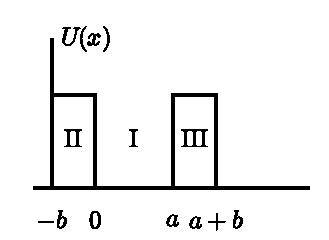
\includegraphics[width=4.5cm]{fig10.pdf}\\[0.3em]
{\small 图\ 10}
\end{minipage}\par\nopagebreak

\begin{equation}\tag{3}
\psi=\mathrm e^{\mathrm i k(a+b)}\bigl[c_3\mathrm e^{\mathrm i\kappa_2(x-a-b)}+c_4\mathrm e^{-\mathrm i\kappa_2(x-a-b)}\bigr]
\end{equation}
$\psi$和$\psi'$在点$x=0$和$x=a$的连续性条件，对于$c_1,\cdots,c_4$给出四个方程；这些方程的相容性条件导致色散方程
\begin{equation}\tag{4}
\cos k(a+b)=\cos\kappa_1 a\cdot\cos\kappa_2 b
-\frac{1}{2}\Bigl(\frac{\kappa_1}{\kappa_2}+\frac{\kappa_2}{\kappa_1}\Bigr)\sin\kappa_1 a\cdot\sin\kappa_2 b.
\end{equation}
这个方程不是以显形式确定待求的关系$\varepsilon(k)$. 在$\varepsilon<U_0$时，$\kappa_2$为虚值，于是方程应写成下列形式
\begin{equation}\tag{5}
\cos k(a+b)=\cos\kappa_1 a\cdot\cosh|\kappa_2 b|
+\frac{1}{2}\Bigl(\frac{|\kappa_2|}{\kappa_1}-\frac{\kappa_1}{|\kappa_2|}\Bigr)\sin\kappa_1 a\cdot\sinh|\kappa_2 b|\,.
\end{equation}
如果在(5)式中，在$U_0b=$常数$\equiv Pa$条件下取极限$U_0\to\infty$，$b\to0$，则得色散方程
\begin{equation}\tag{6}
\cos ka=\cos\kappa_1 a+\frac{Pma^2\sin\kappa_1 a}{\hbar^2\kappa_1 a}.
\end{equation}
这个方程解决了$\delta$函数各峰组成的周期场
\begin{equation*}
U(x)=aP\sum_{a}\delta(x-an)
\end{equation*}
内的能谱问题. 在图11上用图解法给出方程(6)的根的分布. 这里描绘的是方程右侧作为$\kappa_1 a$的函数的图像. 当函数取遍$\pm1$间的所有值时，方程的根值跑遍横轴上粗线段所表示的区域.

\par\nopagebreak\noindent\begin{minipage}{\linewidth}\centering
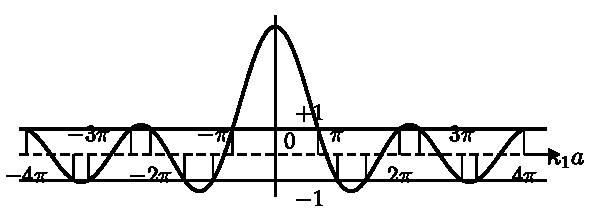
\includegraphics[width=8.5cm]{fig11.pdf}\\[0.3em]
{\small 图\ 11}
\end{minipage}\par\nopagebreak

2. 试求弱周期场$U(x)$内粒子一维运动的色散规律.

{\heiti 解：}将场看作微扰，从零级近似出发，粒子进行以平面波
\begin{equation*}
\psi^{(0)}(x)=(Na)^{-1/2}\,\mathrm e^{\mathrm i kx}
\end{equation*}
描写的自由运动（归一化取成在$Na$长度上有一个粒子，$a$是场的周期）；粒子的能量$\varepsilon^{(0)}=\hbar^2k^2/2m$. 将周期场$U(x)$表示成傅里叶级数的形式：
\begin{equation*}
U(x)=\sum_{-\infty}^{\infty}U_n\mathrm e^{2\pi\mathrm i nx/a}
\end{equation*}
这个场对平面波所取的矩阵元只在波矢为$k$和$k'=k+2\pi n/a$的态间跃迁才不为零，此时$U_{k'k}=U_n$.

在微扰论的一级近似下，能量的修正是由一与$k$无关的常量对角矩阵元$\varepsilon^{(1)}=U_{kk}=U_0$给出的，即能量的原点只作位移而已. 但是，在$k=\pi n/a$（$n=\pm1,\pm2,\cdots$）值的邻域，能级是个例外，在这些点上$k$与$k'=k-2\pi n/a$的值只差一符号. 因此，能量$\varepsilon^{(0)}(k)$和$\varepsilon^{(0)}(k')$是一致的. 于是，在这些值的邻域中，能量相近状态之间的跃迁矩阵元不为零. 为了定出修正值，就需要借助于本征值相近情形的微扰论方法（参阅第三卷§79），第三卷的(79.4)式给出答案. 根据该公式，现在有
\begin{equation*}
\begin{aligned}
\varepsilon_n(k)={}&\frac{1}{2}\bigl[\varepsilon^{(0)}(k)+\varepsilon^{(0)}(k-K_n)\bigr]\pm\\
&\pm\Bigl\{\frac{1}{4}\bigl[\varepsilon^{(0)}(k)-\varepsilon^{(0)}(k-K_n)\bigr]^2+|U_n|^2\Bigr\}^{1/2},
\end{aligned}
\end{equation*}
其中$K_n=2\pi n/a$，并删去了可加常数$U_0$；平方根前符号的选择应满足如下的要求：当远离$k=\pm k_n/2$值时，函数$\varepsilon(k)$应过渡到$\varepsilon^{(0)}(k)$. $+$号和$-$号分别对应于值域$|k|>|k_n/2|$和$|k|<|k_n/2|$，在点$k=\pm k_n/2$上函数$\varepsilon(k)$经历数值为$2|U_n|$的跳跃. 在图12a上，描绘出的能量$\varepsilon(k)$是作为变量$k$的函数，$k$的取值范围为$-\infty$到$\infty$. 如果将$k$值（准动量）取在$\pm\pi/a$之间，就得到图12b，其中绘出头两条能带.

\par\nopagebreak\noindent\begin{minipage}{\linewidth}\centering
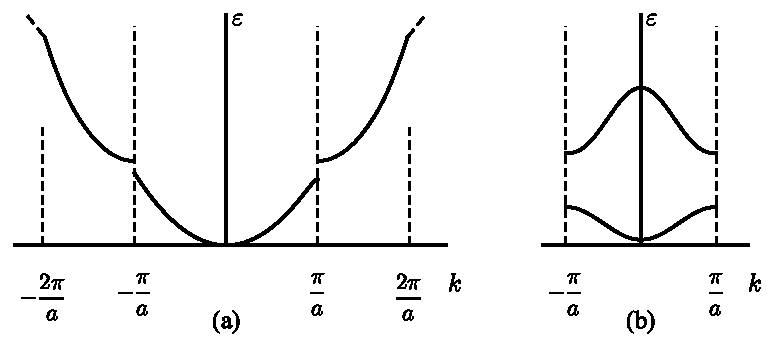
\includegraphics[width=10cm]{fig12.pdf}\\[0.3em]
{\small 图\ 12}
\end{minipage}\par\nopagebreak

我们注意到图12（同图11一样）的能带并不交叠，这是周期场中一维运动的普遍特性. 每个能级（按$k$的符号）是二重简并的，在一维运动时完全不能出现更大的简并度. 我们还要指出，在一维运动情况，每个能带的边界［能量$\varepsilon(k)$的最小值和最大值］对应于数值$k=0$和$k=\pi/a$. 这是因为，在禁戒区间相对应的能量，其波函数在平移一个周期$a$时，需乘以某一实数因子（因此在无穷远处波函数变为无穷大），而在能量的允许区间，在平移时，波函数需乘以因子$\mathrm e^{\mathrm i ka}$. 于是，在禁戒区间和允许区间之间的边界上，这个因子应同时为模等于1的实数. 由此得出$ka$等于零或等于$\pi$.

3. 试求下述一维周期场内粒子的色散规律，这个场是满足准经典条件的一列对称势阱（因此粒子透过势阱间势垒的概率很小）.

{\heiti 解：}类似求解双势阱中能级分裂（第三卷§50习题3）问题的步骤. $\psi_0(x)$是描写在一个势阱中运动（具有某一能量$\varepsilon_0$，图13）的归一化波函数，也就是说从势阱两侧离开边界时波函数按指数函数衰减；这个函数是实函数，而且可以是变量$x$的偶函数或奇函数. 对于周期场内运动的粒子，正确的零级近似波函数是求和式

\par\nopagebreak\noindent\begin{minipage}{\linewidth}\centering
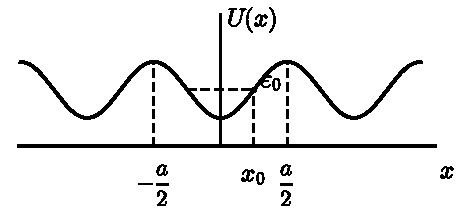
\includegraphics[width=7cm]{fig13.pdf}\\[0.3em]
{\small 图\ 13}
\end{minipage}\par\nopagebreak

\begin{equation}\tag{1}
\psi_k(x)=C\sum_{-\infty}^{\infty}\mathrm e^{\mathrm i kna}\psi_0(x-an),
\end{equation}
其中$C$是归一化常数（当平移$x\to x+a$时，这个函数应该乘以因子$\mathrm e^{\mathrm i ka}$）.

写出薛定谔方程
\begin{equation*}
\begin{aligned}
&\psi''_k+\frac{2m}{\hbar^2}\bigl[\varepsilon(k)-U(x)\bigr]\psi_k=0,\\
&\psi''_0+\frac{2m}{\hbar^2}\bigl[\varepsilon_0-U(x)\bigr]\psi_0=0.
\end{aligned}
\end{equation*}
第一个方程乘以$\psi_0$，第二个方程乘以$\psi_k$，逐项相减，并在界限$-a/2,a/2$内（图13）对$\mathrm dx$积分. 我们指出，因为乘积$\psi_0(x)\psi_0(x-an)$在$n\neq0$时处处很小，那么
\begin{equation*}
\int_{-a/2}^{a/2}\psi_k(x)\psi_0(x)\,\mathrm dx\approx C.
\end{equation*}
我们得出
\begin{equation*}
\varepsilon(k)-\varepsilon_0=\frac{\hbar^2}{2mC}
\bigl[\psi'_0\psi_k-\psi_0\psi'_k\bigr]_{-a/2}^{a/2}.
\end{equation*}
在求和式(1)中，当$x=a/2$时应当只保留$n=0$和$n=1$的项，并且根据函数$\psi_0(x)$的偶奇性$\psi_0(-a/2)=\pm\psi_0(a/2)$，有
\begin{equation*}
\begin{aligned}
&\psi_k(a/2)=C\psi_0(a/2)(1\pm\mathrm e^{\mathrm i ka}),\\
&\psi'_k(a/2)=C\psi'_0(a/2)(1\mp\mathrm e^{\mathrm i ka}).
\end{aligned}
\end{equation*}
同样，在$x=-a/2$时，只应保留$n=0$和$n=1$的项. 结果得到
\begin{equation*}
\varepsilon(k)-\varepsilon_0=\pm\frac{2\hbar^2}{m}\psi_0\Bigl(\frac{a}{2}\Bigr)\psi'_0\Bigl(\frac{a}{2}\Bigr)\cos ka.
\end{equation*}
这里尚需代入值
\begin{equation*}
\begin{aligned}
&\psi_0\Bigl(\frac{a}{2}\Bigr)=\Bigl[\frac{m\omega}{2\pi p(a/2)}\Bigr]^{1/2}
\exp\Bigl[-\frac{1}{\hbar}\int_{x_0}^{a/2}|p(x)|\,\mathrm dx\Bigr],\\
&\psi'_0\Bigl(\frac{a}{2}\Bigr)=\frac{p(a/2)}{\hbar}\psi_0\Bigl(\frac{a}{2}\Bigr).
\end{aligned}
\end{equation*}
其中$\omega$是粒子在势阱中振动的经典频率；$x_0$是与能量$\varepsilon_0$对应的反转点. 最后得到
\begin{equation*}
\varepsilon(k)-\varepsilon_0=\pm\frac{\hbar\omega}{\pi}\sqrt{D}\cos ka,\quad
D=\exp\Bigl[-\frac{4}{\hbar}\int_{x_0}^{a/2}|p(x)|\,\mathrm dx\Bigr].
\end{equation*}
这样一来，在孤立势阱中运动粒子的每一能级$\varepsilon_0$，将展成宽度为$2\hbar\omega D^{1/2}/\pi$的细能带，这个宽度决定于两个势阱间势垒的透射系数$D$.

\end{xiti}

\section{外场对晶格中电子运动的影响}

我们研究晶格上施以一恒定磁场$\bm H$时电子的运动. 在坐标表象内，电子在周期场$U(\bm r)$内的哈密顿量为
\begin{equation}
\hat H=\frac{\hat{\bm p}^2}{2m}+U(\bm r).
\label{56.1}
\end{equation}
（其中$\hat{\bm p}=-\mathrm i\hbar\nabla$是真实动量的算符），由此出发，按通常方式引进外磁场后
\begin{equation}
\hat H=\frac{1}{2m}\Bigl(\hat{\bm p}-\frac{e}{c}\bm A\Bigr)^2+U(\bm r),
\label{56.2}
\end{equation}
其中$\bm A(\bm r)$是场的矢势. 但是，在场足够弱的情况下，过渡到准动量表象，可以使问题得到合理的简化.

鉴于晶格中电子能带结构可以有多种多样的形式，因此只能以相当粗糙的方法对于弱外场的条件进行一般的描述. 设电子在施加外场之前处于某个确定的（第$s$个）能带中，我们用$\varepsilon_0$表示作为这个能带特征的能量最低值，例如，能带的特征宽度或到邻近能带的距离［即给定$\bm k$时的差值$\varepsilon_s(\bm k)-\varepsilon_{s'}(\bm k)$］. 如果认为磁场是弱场，无论如何必须满足条件
\begin{equation}
\hbar\omega_H\ll\varepsilon_0,
\label{56.3}
\end{equation}
其中“拉摩频率”$\omega_H\sim|e|H/m^{*}c$，而$m^{*}\sim\hbar k/v$是电子的有效质量.\footnote{频率更精确的定义由后面公式(57.7)给出. 对于金属中的传导电子（参阅后面的§61）特征值$k\sim1/a$（$a$是晶格常数）；再取$\varepsilon_0\sim\hbar^2/m^{*}a^2$，我们得到与不等式$r_H\gg a$等价的条件(56.3)，其中“轨道半径”$r_H\sim v/\omega_H$.}

如已述及，在无外场时晶格中电子在$\bm k$表象的哈密顿量是元素为$\varepsilon_s(\bm k)$的对角矩阵. 在有外场时，电子的哈密顿量还将包含矢势$\bm A(\bm r)$及其对坐标的微商，即场强$\bm H$（而在非均匀场时，还有场强的高阶微商）；在$\bm k$表象中函数$\bm A(\bm r)$改为算符$\hat{\bm A}=\bm A(\hat{\bm r})$，其中$\hat{\bm r}$算符由(55.14)式给出.

矢势$\bm A(\bm r)$是坐标的增函数（对于均匀场，遵从线性规律）. 鉴于势的这种增长，甚至对于弱场，势在无限大系统（晶格中的电子）的哈密顿量中也不是微扰. 因此，即使弱磁场也会明显改变广延系统的性质——使连续谱变成离散谱（能级量子化，参阅§58）. 而弱场（不同于势）的强度只带来小的修正项.

我们指出，在忽略这些修正项时，只由一些规范不变性的要求便可用一般形式阐明哈密顿量同场势的关系. 因我们研究的是恒定场，所以当势和波函数进行与时间无关的变换
\begin{equation}
\bm A\to\bm A+\nabla\bm f,\quad
\psi\to\psi\exp\Bigl(\frac{\mathrm i e}{\hbar c}\bm f\Bigr)
\label{56.4}
\end{equation}
时，利用方程的不变性就足够了. 这里$\bm f(\bm r)$是坐标的任意函数［参阅第三卷(111.8-9)式］.

在弱场中，势$\bm A(\bm r)$是坐标的缓变函数. 由于要阐述这个缓变性所起的作用，我们首先研究恒定势场这种极限情况：$\bm A(\bm r)=$常量$=\bm A_0$（当然，恒定势是虚构的，此时不存在真实的场，因此谈到的是一个形式的变换）. 从$\bm A=0$过渡到$\bm A=\bm A_0$等价于$\bm f=\bm A_0\cdot\bm r$时的变换(56.4)；因此代替原来（在$\bm A=0$时）本征函数
\begin{equation}
\psi_{s\bm k}=u_{s\bm k}\,\mathrm e^{\mathrm i\bm k\cdot\bm r}
\label{56.5}
\end{equation}
的是新哈密顿量的本征函数
\begin{equation*}
u_{s\bm k}(\bm r)\exp\Bigl\{\mathrm i\Bigl(\bm k+\frac{e}{\hbar c}\bm A_0\Bigr)\bm r\Bigr\}.
\end{equation*}
由此可见，为了赋予准动量以原来的意义（平移时决定波函数相位改变的量）必须取$\bm k+e\bm A_0/\hbar c=\bm K$；这样，定义的量$\bm K$可称为广义准动量. 此时，新本征函数写为
\begin{equation*}
\psi_{s\bm K}=u_{s,\bm K-e\bm A_0/\hbar c}(\bm r)\,\mathrm e^{\mathrm i\bm K\cdot\bm r}.
\end{equation*}
与这些函数相对应的电子能量为：$\varepsilon_s(\bm k)=\varepsilon_s(\bm K-e\bm A_0/\hbar c)$. 现在我们能够断定：势$\bm A(\bm r)$虽非恒定，但在空间缓慢变化时，“零级”波函数近似（对场强而言）是
\begin{equation}
\psi_{s\bm K}=u_{s,\bm K-e\bm A(\bm r)/\hbar c}\,\mathrm e^{\mathrm i\bm K\cdot\bm r}.
\label{56.6}
\end{equation}
（由于$\bm A$是变化的，$u$已经不是严格的周期函数）.\footnote{如果按函数系$\psi_{s\bm k}$展开函数(56.6)，那么，一般说来，在展开式内要包括不同$s$的函数. 但是，应强调指出，这决不意味着真跃迁到另一个能带，而只表明波函数在恒定场影响下的变化；由此联想到，恒定场根本不会引起使能量改变的真实跃迁. 为阐明这种情况，应注意到：虽然场是微弱的，但与此相关的态分类的改变（其中包括准动量与能量的对应）却是明显的.}现在，能量$\varepsilon_s(\bm K-e\bm A/\hbar c)$应当看成是在$\bm K$表象构成哈密顿量的算符. 此时，在同样的近似下，应把$\hat{\bm r}$理解为算符$\hat{\bm r}=\mathrm i\partial/\partial\bm K$，而把定义式(55.14)中第二项$\hat{\bm\Omega}$删去. 实际上，算符$\mathrm i\partial/\partial\bm K$作用于波函数时，按数量级看，是用“轨道线度”$r_H$乘以波函数. 而$r_H$随场的减弱而增大，至于算符$\hat{\bm\Omega}$作用于波函数，其结果并不包含这种增大的因子. 在这个意义上，算符$\hat{\bm\Omega}$在弱场中较$\mathrm i\partial/\partial\bm K$小. 另一方面，因为算符$\partial/\partial\bm K$按能带序号是对角的，则哈密顿量也是对角的.

这样，我们得出结论：晶格中的电子于弱磁场（在$\bm K$表象中）用哈密顿量
\begin{equation}
\hat H_s=\varepsilon_s\Bigl[\bm K-\frac{e}{\hbar c}\bm A(\bm r)\Bigr],\quad
\hat{\bm r}=\mathrm i\frac{\partial}{\partial\bm K}
\label{56.7}
\end{equation}
来描述（R. Peierls, 1933）. 于是，在这个近似下完全类似于在动量表象内自由粒子的哈密顿量中引进磁场的方法.

因为不能确定不可对易算符（矢量$\hat{\bm k}=\bm K-e\hat{\bm A}/\hbar c$的分量）的作用顺序，所以(56.7)还不能完全确定. 而作用顺序的确定应该保证哈密顿量的厄米性. 原则上总是可以做到的，只要把（在倒格子中的）周期函数$\varepsilon_s(\bm k)$展成傅里叶级数型
\begin{equation}
\varepsilon_s(\bm k)=\sum_{\bm a}A_{s\bm a}\,\mathrm e^{\mathrm i\bm k\cdot\bm a}
\label{56.8}
\end{equation}
即可（按正格子的所有矢量$\bm a$求和）. 在这个级数的每一项的指数函数里用$\hat{\bm k}$代替$\bm k$，将只剩下一个算符（矢量$\hat{\bm A}$在$\bm a$上的投影）. 因此不出现作用顺序问题，一切都归结于这一算符的幂. 当然，这样的“厄米化”方法不是唯一的. 然而，重要的在于不同方法间的差别已超出所考虑的近似范围. 因为在上述的近似中，算符$\hat k_x,\hat k_y,\hat k_z$的对易子都是小量. 例如，对于均匀场算符
\begin{equation}
\hat{\bm A}=\frac{1}{2}\bm H\times\hat{\bm r}
=\frac{\mathrm i}{2}\bm H\times\frac{\partial}{\partial\bm K}
\label{56.9}
\end{equation}
容易直接计算出来. 对易子
\begin{equation}
\hat k_x\hat k_y-\hat k_y\hat k_x=\mathrm i\frac{e}{\hbar c}H_z,\cdots
\label{56.10}
\end{equation}
正比于微小场强$\bm H$.

算符$\hat{\bm r}=\mathrm i\partial/\partial\bm K$与$\hat{\bm K}\equiv\bm K$的对易规则和“自由”粒子（无晶格）的坐标与广义动量的对易规则完全一样. 因此计算算符$\hat{\bm r}$和$\hat{\bm K}$与哈密顿量的对易子，自然导致算符方程
\begin{equation}
\hbar\dot{\hat{\bm K}}=-\frac{\partial\hat H}{\partial\hat{\bm r}},\quad
\dot{\hat{\bm r}}=\frac{\partial\hat H}{\hbar\partial\bm K}
\label{56.11}
\end{equation}
这组方程具有通常的哈密顿方程的形式［其计算可参阅第三卷的公式(16.4-5)］.

我们再说一遍，(56.7)式的哈密顿量近似的含意，是其中忽略了与场强$\bm H$有关的各项以及不含数量级为轨道线度$r_H$的大因子项. 在高级的近似中，结果还可以表示为某个有效的哈密顿量$\hat H_s(\bm K-e\hat{\bm A}/\hbar c,\bm H)$的形式，它按能带序号是对角的，并且已经不能仅通过函数$\varepsilon_s(\bm k)$来表达\footnote{计算修正项的简单例子将在§59中给出. 以$\bm H$的幂级数形式得到哈密顿量的正规方法，以及此级数带头项的一般表式在论文：B. I. Blount, Phvs. Rev. 126, 1636 (1962); Soliod State Physics, 卷13, 页306 (1963)中都有表述. 我们指出，如果晶体具有反演中心，则级数始于$\bm H^2$项（参阅§59）.}.

在忽略自旋-轨道相互作用时，计及电子自旋将使哈密顿量中出现通常描述磁矩同场的相互作用的项$-\beta\bm\sigma\cdot\bm H$，其中$\bm\sigma$是泡利矩阵，而$\beta=|e|\hbar/2mc$是玻尔磁子. 如果晶体具有反演中心，自旋-轨道相互作用只改变电子的磁矩，因此自旋同磁场的相互作用为
\begin{equation}
-\beta\sigma_iH_k\xi_{ik}(\bm k).
\label{56.12}
\end{equation}
实际上，在这种情况下对于同时进行时间反演和空间反射，哈密顿量必须是不变的. 在这种变换下，应该进行$\bm H\to-\bm H$和$\bm\sigma\to-\bm\sigma$的变换而使$\bm k$保持不变. (56.12)式是满足所提要求的普遍表达式. 当然，张量$\xi_{ik}(\bm k)$是不能在普遍形式下进行计算的.

最后，我们讲一讲给晶格施加弱电场$\bm E$时电子的行为. 弱场的条件是指电场中在距离$\sim a$上电子所获得的能量小于特征能量$\varepsilon_0:|e|Ea\ll\varepsilon_0$.

与磁场的情形一样，最起作用的项是含坐标增函数的项，即电场标势$\varphi(\bm r)$的项. 利用类似前面的讨论，也能以一般的形式阐明哈密顿量与$\varphi(\bm r)$的关系. 实际上，施加一个虚构的恒定势$\varphi=\varphi_0$等价于在薛定谔方程中给能量附加一个常数$e\varphi_0$；这个常数项也加在所有的本征值$\varepsilon_s(\bm k)$上. 当势$\varphi(\bm r)$不恒定，但在空间中缓变时，类似的算符项应追加一个$\bm k$表象中的有效哈密顿量：
\begin{equation}
\hat H_s=\varepsilon_s(\bm k)+e\varphi(\hat{\bm r}).
\label{56.13}
\end{equation}

\section{准经典轨道}

我们把上节获得的结果运用到电子在磁场中进行准经典运动这一重要情况. 如所周知，准经典条件是：粒子的德布罗意波长在粒子的线度上变化很小. 现在，这个条件等价于不等式：
\begin{equation}
r_H\gg\lambda,
\label{57.1}
\end{equation}
即轨道的曲率半径远大于波长$\lambda\sim1/k$\footnote{一般说来，这个条件强于条件(56.3). 但如果$k\sim1/a$（金属中传导电子就是这种情况），则两个条件变为一致. 而且，实际上总可以得到满足. 在$r_H\sim c\hbar k/|e|H\sim c\hbar/a\,|e|H$时，条件$r_H\gg a$导致要求$H\ll c\hbar/|e|a^2\sim10^8-10^9\,$Oe（奥斯特）.}.

在准经典条件下，粒子轨道的概念便有意义了. 轨道由运动方程来确定，而运动方程是用相应的经典量
\begin{equation*}
\hbar\dot{\bm K}=-\frac{\partial H}{\partial\bm r},\quad
\bm v=\frac{\partial H}{\hbar\partial\bm K},\quad
H=\varepsilon\Bigl(\bm K-\frac{e}{\hbar c}\bm A(\bm r)\Bigr)
\end{equation*}
代替(56.11)式中的算符而得出的（为了简化略去下标$s$）. 我们展开这些方程，以“动理学的准动量”：
\begin{equation*}
\bm k=\bm K-\frac{e}{\hbar c}\bm A(\bm r)
\end{equation*}
替换广义准动量$\bm K$.

我们有
\begin{equation*}
\frac{\hbar\,\mathrm d\bm k}{\mathrm dt}+\frac{e\,\mathrm d\bm A(\bm r)}{c\,\mathrm dt}
=-\frac{\partial H}{\partial\bm r}=\frac{e}{c}\,v_i\frac{\partial A_i}{\partial\bm r}.
\end{equation*}
在此写出$\mathrm d\bm A/\mathrm dt=(\bm v\cdot\nabla)\bm A$，并注意到
\begin{equation*}
(v_i\nabla)A_i-(\bm v\cdot\nabla)\bm A=\bm v\times(\nabla\times\bm A)=\bm v\times\bm H,
\end{equation*}
便获得运动方程
\begin{equation}
\frac{\hbar\,\mathrm d\bm k}{\mathrm dt}=\frac{e}{c}\bm v\times\bm H,\quad
\bm v=\frac{\partial\varepsilon(\bm k)}{\hbar\partial\bm k}
\label{57.2}
\end{equation}
这个方程只由于另一种$\varepsilon(\bm k)$关系而与通常的经典洛伦兹方程不同，其中代替简单的二次函数的是复杂的周期函数；相应地，关系式$\bm v(\bm k)$也是这种复杂的周期函数. 自然，这种情形要使电子运动的性质产生重大变化.

我们研究电子在均匀磁场内的运动，用$\bm v$乘方程(57.2)，用通常的方法求出$\hbar\bm v\cdot\mathrm d\bm k/\mathrm dt=\mathrm d\varepsilon/\mathrm dt=0$. 再用$\bm H$乘方程(57.2). 得到$\mathrm d(\bm H\cdot\bm k)/\mathrm dt=0$. 这样，电子在晶格内运动如同自由电子在磁场内运动一样：
\begin{equation}
\varepsilon=\text{常量},\quad k_z=\text{常量}.
\label{57.3}
\end{equation}
（$z$轴沿磁场$\bm H$的方向）. 等式(57.3)决定电子在$\bm k$空间的轨道. 几何上，这个轨道是垂直于磁场的平面与等能面$\varepsilon(\bm k)=$常量相截的截口曲线.

等能面会有各种形式. 在每个倒格子原胞内，这些等能面可以有几个彼此不相连的叶片. 这些叶片可以是单连通的或是多连通的，可以是闭的或是开的. 为了阐述后一种区别，最好来研究周期地延伸在整个倒格子的等能面. 在每一个倒格子原胞里有相同的闭空腔，而开的等能面连续地通过整个格子并延伸至无穷远\footnote{为避免误解，应当指出，倒格子原胞不能这样选取，即所有本质不同的（即不是周期性重复的）一些闭空腔处在一个原胞内而不被原胞界面截开.}.

等能面的截面由无穷多个截口曲线构成. 这里既包括倒格子一个原胞范围内等能面不同叶片的截口曲线，也包括在不同原胞内重复叶片的截口曲线.

如果等能面的叶片是闭的，那么它的所有截面也都是闭曲线. 如果叶片是开的，那么它的各截面既可以是闭的，也可以是开的（即连续地延伸到整个倒格子）.

运动的准经典性也意味着磁击穿（magnetic breakdown）的概率很小，即电子的准动量不大可能跃变式地从一个截口曲线过渡到另一个截口曲线（在本节最后我们还要讨论磁击穿概率很小的条件）. 于是，当忽略这个可能性时，电子就只在等能面的一个截口曲线上运动.

现在我们详细研究在准动量空间内沿封闭轨道的运动. 显然，这是时间上的周期运动；我们来确定它的周期.

把方程(57.2)投影到与场垂直的平面$k_x,k_y$上，得到
\begin{equation*}
\frac{\mathrm dl_k}{\mathrm dt}=\frac{|e|H}{c\hbar}\,v_{\perp},\quad
v_{\perp}=\sqrt{v_x^2+v_y^2},
\end{equation*}
其中$\mathrm dl_k=\sqrt{\mathrm dk_x^2+\mathrm dk_y^2}$是$\bm k$轨道的线元. 由此得到
\begin{equation*}
t=\frac{c\hbar}{|e|H}\int\frac{\mathrm dl_k}{v_{\perp}}.
\end{equation*}
如果轨道是封闭的，则运动周期由对轨道全路径的积分
\begin{equation}
T=\frac{c\hbar}{|e|H}\oint\frac{\mathrm dl_k}{v_{\perp}}
\label{57.4}
\end{equation}
给出. 这个表达式可用下面的方法变为更直观的形式.

用平面$k_z=$常量截等能面$\varepsilon=$常量，其截面积取为$S(\varepsilon,k_z)$. 在这个平面上两个路径$\varepsilon=$常量和$\varepsilon+\mathrm d\varepsilon=$常量之间的环宽在路径的每一点上是
\begin{equation*}
\frac{\mathrm d\varepsilon}{|\partial\varepsilon/\partial k_{\perp}|}=\frac{\mathrm d\varepsilon}{\hbar v_{\perp}},
\end{equation*}
因而这个环的面积是
\begin{equation*}
\mathrm dS=\mathrm d\varepsilon\oint\frac{\mathrm dl_k}{\hbar v_{\perp}},
\end{equation*}
由此可见，(57.4)式中的积分，正是偏微商$\partial S/\partial\varepsilon$. 于是，运动周期为
\begin{equation}
T=\frac{c\hbar^2}{|e|H}\frac{\partial S(\varepsilon,k_z)}{\partial\varepsilon},
\label{57.5}
\end{equation}
（W. Shockley, 1950）. 在此，自然地引进称为晶格中电子的回旋质量：
\begin{equation}
m^{*}=\frac{\hbar^2\partial S}{2\pi\partial\varepsilon},
\label{57.6}
\end{equation}
电子在轨道上的回转频率通过这个量用公式
\begin{equation}
\omega_H=|e|H/m^{*}c
\label{57.7}
\end{equation}
表出，它同自由电子拉摩频率著名公式的区别只是将质量换成$m^{*}$.\footnote{自由电子的等能面是半径为$\varepsilon=\hbar^2k^2/2m$的球面，它的截面是面积为$S=\pi(2m\varepsilon\hbar^{-2}-k_z^2)$的圆，所以微商$\partial S/\partial\varepsilon=2\pi m/\hbar^2$，因而$m^{*}=m$.}

但是，我们强调指出，晶格中电子的回旋质量不是恒量，而是$\varepsilon$和$k_z$的函数，所以各个电子的回旋质量也不同. 还注意到，这个量可正可负；在前者电子作为荷负电的粒子沿轨道运动，后者是作为荷正电的粒子——空穴——在运动. 与此相应地说成电子轨道和空穴轨道.

到目前为止，我们讲过的是在$\bm k$空间的电子轨道. 但是，容易看出，准动量空间中的轨道和普通空间中的轨道间存在密切的联系. 运动方程(57.2)改写成形式
\begin{equation*}
\hbar\,\mathrm d\bm k=-\frac{|e|}{c}\,\mathrm d\bm r\times\bm H.
\end{equation*}
积分后（适当地选取坐标$\bm r$和准动量$\bm k$的原点）得到
\begin{equation}
\hbar\bm k=-\frac{|e|}{c}\,\bm r\times\bm H.
\label{57.8}
\end{equation}
由此看出，普通空间中轨道的$xy$投影，本质上是$\bm k$轨道的再现，只是取向和比例不同而已；从$\bm k$轨道经变换
\begin{equation*}
k_x\to-\frac{|e|H}{\hbar c}\,y,\quad
k_y\to\frac{|e|H}{\hbar c}\,x,
\end{equation*}
便得出普通空间轨道. 除此之外，在普通空间有以速度$v_z=\partial\varepsilon/\hbar\partial k_z$沿$z$轴的运动. 如果在$\bm k$空间的轨道是封闭的，那么普通空间轨道就是以场方向为轴的螺旋线. 如果轨道是开口的，则甚至在普通空间中轨道在$xy$平面上的投影也是开口的，就是说，在这个平面上运动可通向无限远.

再说一下晶格处于恒定均匀电场$\bm E$中电子的准经典运动. 由准经典方程$\hbar\dot{\bm k}=e\bm E$，我们有
\begin{equation}
\bm k=\bm k_0+\frac{e\bm E}{\hbar}\,t,
\label{57.9}
\end{equation}
再根据能量守恒定律，有
\begin{equation}
\varepsilon(\bm k)-e\bm E\cdot\bm r=\text{常量}.
\label{57.10}
\end{equation}
但是，能量$\varepsilon(\bm k)$是在有限区间$\Delta\varepsilon$（能带宽度）内取值的；因此，从(57.10)式得出，在均匀电场内的电子沿场方向做有限运动：电子在这个方向以振幅$\Delta\varepsilon/|e|E$振动. 如果电场平行于任一个倒格子的周期$\bm b$，则运动就是频率为$\omega=2\pi|e|E/\hbar b$的周期运动；当$b\sim1/a$时，有$\hbar\omega_E\sim|e|Ea$. 对于场方向任意这种一般情况，运动是准周期的.

最后我们讨论前述可以忽略磁击穿的条件. 如果这些轨道在某处反常地接近，那么从一条轨道过渡到另一条轨道（在$\bm k$空间）的概率自然就大. 这样的情况出现在：当轨道与具有自交叉的轨道相接近时，或者轨道在等能面两叶交叉点附近（也就是简并点附近）通过时. 这些情况的轨道的典型图像如图14所示：轨道间的间隙$\delta k$小于整个轨道的特征线度. 而在其最近处的轨道曲率半径$R_k$，一般说来，与$\delta k$同数量级. 借助量子隧道效应可以从一条轨道过渡到另一条轨道. 如果$\delta k$大于距离$\Delta k_x$（在这个距离上，波函数在经典不可到达的轨道之间的区域内要衰减），这个过渡概率不大（按指数函数）.

\par\nopagebreak\noindent\begin{minipage}{\linewidth}\centering
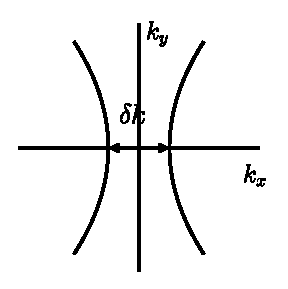
\includegraphics[width=4.5cm]{fig14.pdf}\\[0.3em]
{\small 图\ 14}
\end{minipage}\par\nopagebreak

利用电子在磁场内的运动与在某个势场$U(x)$内的一维运动的相似性可以估计出$\Delta k_x$. 这个相似性来源于：根据(56.10)式，算符$\hat q\equiv\hat k_x\hbar c/|e|H$和$\hat p\equiv\hbar\hat k_y$所满足的对易关系同坐标和动量的对易关系一致. 在最接近点附近，轨道是抛物线. 它们类似于均匀场$(U=-Fx)$中一维运动的抛物线相轨道$(x,p)$，其方程为$p^2/2m=Fx$（如果$x$自转向点算起）. 在这种情况下，在反转点后的距离$\Delta x\sim(\hbar^2/mF)^{1/3}$上的波函数将衰减掉（见第三卷§24）；引入相轨道的曲率半径$R\sim(\mathrm d^2x/\mathrm dp^2)^{-1}\sim mF$，可写出$\Delta x\sim(\hbar^2/R)^{1/3}$. 根据所指出的类似性，可借代换$\Delta x\to\hbar c\Delta k_x/|e|H$，$R\to R_k\hbar|e|H/c$得出待求量$\Delta k_x$. 于是获得$\Delta k_x\sim(|e|H/\hbar c)^{2/3}(\delta k)^{-1/3}$，并且，条件$\Delta k_x\ll\delta k$变为
\begin{equation}
|e|H/\hbar c\ll(\delta k)^2
\label{57.11}
\end{equation}
的形式.

\section{准经典能级}

我们看到，处在外磁场中晶格里的电子在$\bm k$空间沿闭合轨道的经典运动，对应着普通空间中与磁场$\bm H$垂直的平面上的有限运动. 当过渡到量子力学时，在每一个纵向准动量$k_z$的确定值都出现离散的能级. 这些能量值由准经典量子化的一般规则确定.

我们选择均匀磁场（方向沿$z$轴）的矢势形如：$A_x=-Hy$，$A_y=A_z=0$. 这时，广义准动量的分量为
\begin{equation}
K_x=k_x+\frac{|e|}{c\hbar}Hy,\quad K_y=k_y,\quad K_z=k_z,
\label{58.1}
\end{equation}
坐标$x$是循环变量，因此，广义准动量的$x$分量守恒：
\begin{equation}
K_x=k_x+\frac{|e|}{c\hbar}Hy=\text{常量}.
\label{58.2}
\end{equation}
根据玻尔-索末菲量子化规则（参阅第三卷§48），写出条件
\begin{equation}
\frac{1}{2\pi}\Bigl|\oint K_y\,\mathrm dy\Bigr|=n,
\label{58.3}
\end{equation}
这里的积分取运动的一个周期，并假定$n$是大的正整数\footnote{在均匀磁场内运动，与矢势选择无关的浸渐不变量是积分
\begin{equation*}
\frac{1}{2\pi}\oint\bm K_i\cdot\mathrm d\bm r,
\end{equation*}
其中$\bm K_i$是与场垂直平面上的广义准动量的投影（对比第二卷§21）. 矢势$\bm A$在所选的情况下，积分$\oint K_x\,\mathrm dx=K_x\oint\mathrm dx=0$，所以浸渐不变量同(58.3)式中的积分一致.} 根据公式(58.1-2)将$K_y=k_y$和$\mathrm dy=-(c\hbar/|e|H)\mathrm dk_x$代入，我们得到
\begin{equation}
\frac{c\hbar}{2\pi|e|H}\Bigl|\oint k_y\,\mathrm dk_x\Bigr|=n.
\label{58.4}
\end{equation}
现在，这里的积分取在$\bm k$空间中的闭合轨道上. 这个积分正是轨道包围的面积，也是前节引入的被平面$k_z=$常量截得等能面的截面积$S(\varepsilon,k_z)$.

于是，最终得到
\begin{equation}
S(\varepsilon,k_z)=2\pi\frac{|e|H}{c\hbar}\,n.
\label{58.5}
\end{equation}
（И.\,М.\,Лифшиц, 1951; L. Onsager, 1952）. 这个条件以非显示的形式确定出能级$\varepsilon_n(k_z)$. 于是，能带（为简单计我们不写出序号$s$）分解为朗道次能带的离散系列，其中各条次能带都是以连续变量$k_z$值来区别的.

如所周知，准经典的量子化条件由于引入一修正项而更加准确，这个修正项归结为对一个大的量子数$n$附加数量级为1的数. 为确定这个修正项，需要考察(58.3)式中限定积分范围的各“转向点”附近的运动.

在电子轨道上$K_y=k_y$与$y$的关系，当给定$k_z$值并在$k_z=$常量时由方程
\begin{equation}
\varepsilon(\bm k)=\varepsilon\Bigl(K_x-\frac{|e|H}{c\hbar}y,\,k_y,\,k_z\Bigr)=\text{常量}
\label{58.6}
\end{equation}
来确定；转向点$y=y_0$由速度$v_y=\partial\varepsilon/\hbar\partial k_y$变为零的条件来确定. 在这点附近，按$y-y_0$的幂展开方程(58.6)而得出
\begin{equation*}
-\frac{|e|H}{c\hbar}\Bigl(\frac{\partial\varepsilon}{\partial k_x}\Bigr)_0(y-y_0)
+\frac{1}{2}\Bigl(\frac{\partial^2\varepsilon}{\partial k_y^2}\Bigr)_0(k_y-k_{y_0})^2=0.
\end{equation*}
其中$k_{y_0}=k_y(y_0)$. 由此可见，按平方根定律
\begin{equation*}
k_y-k_{y_0}=\pm A\sqrt{y-y_0}.
\end{equation*}
来逼近转向点（为明确起见，我们认为经典不可到达区域在$y<y_0$）. 但是，这个定律正是准经典量子化中通常导出修正项的方法（参阅第三卷§47, §48）所涉及的定律. 于是(58.5)的精确规则为
\begin{equation}
S(\varepsilon,k_z)=2\pi\frac{|e|H}{c\hbar}\Bigl(n+\frac{1}{2}\Bigr).
\label{58.7}
\end{equation}
从推导中知道（基于函数(58.6)的展开），为了使精确的量子化规则变得有效，轨道需要充分远离函数$\varepsilon(\bm k)$的各奇点（其中包括复数的支点）. 在轨道附近处处不应破坏准经典条件（特别是速度$\partial\varepsilon/\partial\bm k$的$x,y$投影不要变为零）\footnote{两条轨道反常接近点附近，这些条件与磁击穿概率要小的要求一致.}. 最后，必须注意到作为一切推导基础的哈密顿量(56.7)是近似的. 如果格子有反演中心，哈密顿量的修正项便是场强的二次函数，因而不影响条件(58.7). 但是，若不存在反演中心，哈密顿量的修正项便是$\bm H$的线性函数；在这种情况下，(58.7)中的修正项$1/2$便失去意义，因为哈密顿量的近似性也会造成同数量级的误差.\footnote{对于自由电子（参考225页的注），根据朗道关于磁场中自由电子的著名公式（第Ⅲ卷§112），条件(58.7)给出
\begin{equation*}
\varepsilon=\hbar\omega_H\Bigl(n+\frac{1}{2}\Bigr)+\hbar^2k_z^2/2m,\quad \omega_H=|e|H/mc
\end{equation*}}

两个相邻能级的间隔$\Delta\varepsilon$与大数$n$改变1相对应. 于是$\Delta\varepsilon$由等式
\begin{equation}
\Delta S=\frac{\partial S}{\partial\varepsilon}\Delta\varepsilon=\frac{2\pi|e|H}{\hbar c}
\label{58.8}
\end{equation}
来确定. 引入周期运动的经典频率$\omega_H$，根据(57.7)我们得到
\begin{equation}
\Delta\varepsilon=\hbar\omega_H.
\label{58.9}
\end{equation}
应强调指出，频率$\omega_H$本身是$\varepsilon(n,k_z)$的函数. 因此，相继的能级$\varepsilon_n$（在给定$k_z$时）不是严格等间隔的，这和自由电子情况不一样，在那里$\omega_H$是常数.

能级与守恒量$K_x$无关（与磁场中的自由电子一样——参阅第三卷§112），表明它们是简并的. 如果设想晶格具有大而有限的体积$V$，那么简并度将是有限数. 在区间$\mathrm dk_z$且$n$为给定时，状态数为$V\Delta S\cdot\mathrm dk_z/(2\pi)^3$，其中$\Delta S$是量子数为$n$和$n+1$的两条轨道间所包平面$k_z=$常量的面积. 这个面积由公式(58.8)给出，于是，我们得到所求状态数的表达式
\begin{equation}
\frac{V\,\mathrm dk_z\,|e|H}{(2\pi)^2\,c\hbar},
\label{58.10}
\end{equation}
——这同自由电子情况的公式一样.

在磁场中能级简并的明显原因在于：能量与电子“拉摩轨道中心”在空间内的位置无关. 对于自由电子这个简并是精确的. 对于晶格中的电子它只可能是近似的：这是因为存在非均匀（周期）的电场，在晶格原胞中“轨道中心”的不同位置已不再等价. 这一情况必然导致朗道能级的某些分裂.

考虑电子的自旋将使每个能级分裂成两个；忽略自旋-轨道耦合时，这两个成分被恒定间隔$2\beta H$所分离（如自由电子一样），其中$\beta$是玻尔磁子：
\begin{equation}
\varepsilon_{n\sigma}(k_z)=\varepsilon_n(k_z)+\sigma\beta H,\quad\sigma=\pm1.
\label{58.11}
\end{equation}
如果晶体具有反演中心，当考虑自旋-轨道相互作用时，上述情况仍然成立. 此时，无场存在的电子态对自旋是简并的，而磁场则消除这个简并. 若用$\beta\xi_n(k_z)$替换$\beta$［其中$\xi_n(k_z)$表示电子磁矩的变化］，结果也能得到(58.11)同样的公式.

\section{晶格中电子的有效质量张量}

我们研究$\bm k$空间$\bm k=\bm k_0$的点，在这个点上电子的能量$\varepsilon_s(\bm k)$有极值；特别是，与能带的顶和底对应的点就是这样的点. 如果在这样的点上没有简并（只有对自旋可能存在克拉默斯简并才是例外，参考§55末），那么，在该点附近的函数$\varepsilon_s(\bm k)$可以按差$\bm q=\bm k-\bm k_0$的幂作正则展开. 这样展开的首批项是二次项：
\begin{equation}
\varepsilon_s(\bm k)=\varepsilon_s(\bm k_0)+\frac{\hbar^2}{2}\,m^{-1}_{ik}\,q_iq_k.
\label{59.1}
\end{equation}
(59.1)式中的系数张量$m^{-1}_{ik}$的逆张量是$m_{ik}$，它称为电子在格子中的有效质量张量. 下面来阐明，如何用$k_0$点的布洛赫函数$\psi_{s\bm k_0}$所构成的矩阵元来表示这个张量.

当忽略自旋-轨道相互作用时，电子的哈密顿量是(56.1)式的形式. 我们将
\begin{equation}
\psi_{s\bm k}=\mathrm e^{\mathrm i(\bm k_0+\bm q)\cdot\bm r}u_{s\bm k}\equiv
\mathrm e^{\mathrm i\bm q\cdot\bm r}\varphi_{s\bm k}
\label{59.2}
\end{equation}
形式的波函数代入此哈密顿量的薛定谔方程. 此时方程为
\begin{equation}
\Bigl\{-\frac{\hbar^2}{2m}\Delta+U(\bm r)
+\Bigl[\frac{\hbar}{m}\bm q\cdot\hat{\bm p}+\frac{\hbar^2q^2}{2m}\Bigr]\Bigr\}\varphi_{s\bm k}
=\varepsilon_s(\bm k)\varphi_{s\bm k},
\label{59.3}
\end{equation}
其中$\hat{\bm p}=-\mathrm i\hbar\nabla$，是真实动量的算符.

在$\bm k=\bm k_0$点的附近，矢量$\bm q$是个小量，因此(59.3)式方括号里的表达式可以看成微扰算符. 在零级近似，当$\bm q=0$时函数$\varphi_{s\bm k}$同函数$\varphi_{s\bm k_0}$一致. 因此，通常的微扰理论可以通过此函数所构成的矩阵元来表达对能量的修正.

因为$\bm k_0$是极值点，就不存在关于$\bm q$的线性修正项. 就是说，对角矩阵元等于零，即
\begin{equation}
\langle s\bm k_0|\bm p|s\bm k_0\rangle=0.
\label{59.4}
\end{equation}
为了确定关于$\bm q$的二次修正项，必须考虑一级微扰算符中$q^2$的项，以及二级微扰论中$\bm q$的项. 结果得到$\varepsilon_s(\bm k)$的公式(59.1)，其中
\begin{equation}
m^{-1}_{ik}=\frac{\delta_{ik}}{m}+\frac{1}{m^2}\sum_{s'}^{\prime}
\frac{(\bm p_i)_{ss'}(\bm p_k)_{s's}+(\bm p_k)_{ss'}(\bm p_i)_{s's}}
{\varepsilon_{s'}(\bm k_0)-\varepsilon_s(\bm k_0)}
\label{59.5}
\end{equation}
按所有$s\neq s'$进行求和\footnote{不存在按$\bm k'$的求和，因为根据(55.15)式，动量$\bm p=m\bm v$没有对于$\bm k$的非对角矩阵元，因此所有的中间态都与同一个准动量$\bm k_0$有关.}. 为了简化对矩阵元的描述，这里和今后将略去对角指标$\bm k_0: \bm p_{ss'}\equiv\langle s\bm k_0|\bm p|s'\bm k_0\rangle$. 我们指出，若能带靠得近时（即$\varepsilon_{s'}-\varepsilon_s$是小量），(59.5)的第二项可以大于第一项，由此有效质量将小于$m$.

现在假设给晶体施加一均匀磁场$\bm H$. 这时，在(59.1)中用算符
\begin{equation}
\hat{\bm q}=\bm Q-\frac{e}{\hbar c}\hat{\bm A},\quad
\hat{\bm A}=\frac{1}{2}\bm H\cdot\mathrm i\frac{\partial}{\partial\bm Q},
\label{59.6}
\end{equation}
替换$\bm q$，根据(56.7)式便得到哈密顿量：
\begin{equation}
\hat H^{(0)}_s=\varepsilon_s(\bm k_0)+\frac{\hbar^2}{2}\,m^{-1}_{ik}\,\hat q_i\hat q_k.
\label{59.7}
\end{equation}
它作用在广义准动量$\bm Q$的函数上，自然它与原来的公式(59.1)有同样适用的能量区域. 这就是说，除掉弱场条件(56.3)外，还假设所研究的朗道能级的位置不很高. 在这个意义上，应该将$\bm q$和$\bm Q$这两个量看成是小量（甚至在弱场，矢势$\bm A$也有增大的特点，不能认为$\bm A$小于$\bm Q$）.

哈密顿量中在(59.7)式以后的各项均包含“纯粹”形式的$\bm H$场（即不伴有算符$\partial/\partial\bm Q$）. 这样一些项已经不能只从规范不变性的考虑中得到. 我们来确定这些项中的首项，它是$\bm H$的线性项. 此时，由于这个线性项较小，在计算它的时候可以假定$\bm Q=0$.

首先在不考虑自旋-轨道相互作用时，我们来研究所提出的课题. 我们所感兴趣的是$\bm H$的线性项，它只可能在电子的原始的精确哈密顿量(56.2)中关于$\bm A$的线性项里出现，就是说它出现在用波函数$\psi_{s\bm k_0}$对表达式
\begin{equation}
-\frac{e}{2mc}\bigl(\hat{\bm p}\cdot\bm A+\bm A\cdot\hat{\bm p}\bigr)
=-\frac{e}{mc}\bm A\cdot\hat{\bm p}
\label{59.8}
\end{equation}
的求平均中（等式与已选的$\nabla\cdot\bm A=0$的规范有关）. 这在哈密顿量(59.7)中导致附加项
\begin{equation}
H^{(1)}_s=-\bm M\cdot\bm H,
\label{59.9}
\end{equation}
其中
\begin{equation}
\bm M=\frac{e}{2mc}\bigl\langle s\bm k_0|\bm r\times\bm p|s\bm k_0\bigr\rangle,
\label{59.10}
\end{equation}
正好是电子在态$s\bm k_0$上磁矩的平均值. 我们强调指出，修正项(59.9)可以附加在哈密顿量(59.7)上，而不必担心这个效应已经部分地在(59.6)的替换中考虑到了；事实上,式(59.7)中$\bm H$的线性项在$\bm Q=0$时根本不存在.

考虑到(59.4)式，$\bm p$不存在对角矩阵元，按照矩阵乘法规则我们把式(59.10)分开写出得
\begin{equation*}
\bm M_x=\frac{e}{2mc}\sum_{s'}^{\prime}
\bigl[(\bm\Omega_y)_{ss'}(\bm p_z)_{s's}-(\bm\Omega_z)_{ss'}(\bm p_y)_{s's}\bigr],
\end{equation*}
（对于$\bm M_y,\bm M_z$也类似）；情况正应如此，哈密顿量(59.7)的修正项通过算符$\bm\Omega$的矩阵元来表示. 借助关系式
\begin{equation*}
\bm\Omega_{s's}=\frac{\bm p_{s's}}{\mathrm i(\varepsilon_{s'}-\varepsilon_s)},
\end{equation*}
可将$\bm M$改写成如下形式
\begin{equation}
\bm M_x=\frac{\mathrm ie}{2mc}\sum_{s'}^{\prime}
\frac{(\bm p_z)_{ss'}(\bm p_y)_{s's}-(\bm p_y)_{ss'}(\bm p_z)_{s's}}
{\varepsilon_{s'}(\bm k_0)-\varepsilon_s(\bm k_0)},\cdots
\label{59.11}
\end{equation}
我们注意到，如果晶体具有反演中心，那么，$\bm M$以及整个修正式(59.9)都变为零. 事实上，同时进行时间反演和空间反演，电子的状态（不考虑自旋时）是不变的，因此等式(59.11)的右侧也就不变；而磁矩在此变换下应该变号.

现在，我们计及晶体中的自旋-轨道相互作用，给哈密顿量(56.1)附加(55.17)的自旋-轨道项$\hat H_{sl}$，这将改变方程(59.3)中关于$\bm q$的线性项：在这一项中算符$\hat{\bm p}$变成
\begin{equation}
\hat{\bm\pi}=\hat{\bm p}+\frac{\hbar}{4mc^2}\bm\sigma\times\nabla U.
\label{59.12}
\end{equation}
算符$\hat{\bm\pi}$有简单的物理意义：哈密顿量（包括$\hat H_{sl}$）同$\bm r$直接对易，无磁场时我们得到
\begin{equation}
\hat{\bm r}=\frac{\hat{\bm\pi}}{m}.
\label{59.13}
\end{equation}
类似地，当有磁场时，在原来的哈密顿量（也包括$\hat H_{sl}$）中进行通常的代换$\hat{\bm p}\to\hat{\bm p}-e\bm A/c$，我们得到关于$\bm A$的线性项形如$-e\hat{\bm\pi}\cdot\bm A/mc$，它跟(59.8)的区别也是将$\hat{\bm p}$换成$\hat{\bm\pi}$. 对磁矩(59.11)还应追加一项自由电子的自旋磁矩，因此有
\begin{equation}
\bm M_x=\beta\langle s\bm k_0|\sigma_x|s\bm k_0\rangle+\frac{\mathrm ie}{2mc}\sum_{s'}^{\prime}
\frac{(\bm\pi_z)_{ss'}(\bm\pi_y)_{s's}-(\bm\pi_y)_{ss'}(\bm\pi_z)_{s's}}{\varepsilon_{s'}-\varepsilon_s}
\label{59.14}
\end{equation}
考虑到自旋-轨道相互作用，这个表达式的第二项甚至在有反演中心的晶体里也绝不等于零. 事实上，时间和空间同时改变符号会导致自旋方向相反的状态. 因此，如果在这种变换时改变符号，整个表达式(59.14)仅应归结为对算符$\beta\sigma_i\xi_{ix}(\bm k)$的平均（对照(56.12)式）.

当自旋-轨道相互作用可以看成微扰时，\footnote{$\hat H_{sl}$的表达式(55.17)是按相对论比值$(v/c)^2$展开的第一项. 因此，在一定意义上它总是小量. 但是，这个微小性对于现在这个具体能带中运用微扰论并无关系. 因此$\hat H_{sl}$在所研究的问题里并不能总认为是小的微扰.}我们来计算张量$\xi_{ik}$. 改写(55.17)如下列形式
\begin{equation}
\hat H_{sl}=\bm\sigma\cdot\hat{\bm\chi},\quad
\hat{\bm\chi}=\frac{\mathrm i\hbar^2}{4m^2c^2}\nabla U\times\nabla.
\label{59.15}
\end{equation}
把(59.9)和(59.15)看成微扰，我们来求能量的二级微扰论的修正项，此时只剩下对于(59.9)和(59.15)的交叉项. 这个修正项（仍然是一个关于自旋变量的算符——矩阵）具有(56.12)的形式，其张量$\xi_{ik}$等于
\begin{equation}
\xi_{ik}=\delta_{ik}+\frac{1}{2}\sum_{s'}^{\prime}
\frac{(\bm\chi_i)_{ss'}(\bm L_k)_{s's}+(\bm L_k)_{ss'}(\bm\chi_i)_{s's}}
{\varepsilon_{s'}-\varepsilon_s}
\label{59.16}
\end{equation}
其中$\hbar\hat{\bm L}=\bm r\times\hat{\bm p}$.

上述一切都是关于自旋以外的非简并态的. 如果在$\bm k=\bm k_0$时有简并，那么，为了确定能量，需要组成直到二级微扰［方程(59.3)中的方括号］的久期方程（即根据第三卷公式(39.4)）. 如此，得出的久期方程的性质与$\bm k_0$点的对称性有关. 我们在§68还要讨论这个问题.

\begin{xiti}

粒子在任意方向的磁场内具有平方色散律(59.1)，试求其准经典能级.

{\heiti 解：}将张量$m_{ik}$化为对角型，并从极值点（为明确起见取极小值）开始计算能量和动量. 这时
\begin{equation}\tag{1}
\varepsilon(\bm k)=\frac{\hbar^2}{2}\Bigl(\frac{k_1^2}{m_1}+\frac{k_2^2}{m_2}+\frac{k_3^2}{m_3}\Bigr).
\end{equation}
其中$m_1,m_2,m_3$是张量$m_{ik}$的主值（正值），用$\bm n$表示场$\bm H$方向的单位矢，有
\begin{equation}\tag{2}
k_z=\bm n\cdot\bm k=n_1k_1+n_2k_2+n_3k_3
\end{equation}
（$n_1,n_2,n_3$是场对张量$m_{ik}$主轴的方向余弦），我们需要求出平面(2)在椭球体(1)内那部分的面积；它可以表成对椭球体(1)取的积分：\footnote{令$f(x,y,z)=$常量是填充某一体积的曲面族. $\mathrm dl$是曲面族内两个无限接近曲面间的距离：$\mathrm dl=\mathrm df/|\bm\nabla f|$，这两个曲面间的体积$\mathrm dV=S(f)\,\mathrm dl$，其中$S(f)$是给定$f$值的曲面面积. 以$\delta$函数$\delta(f)$乘以等式$S(f)\,\mathrm df=|\bm\nabla f|\,\mathrm dV$，再对体积取按$\mathrm df$的积分，于是得曲面$f(x,y,z)=0$的面积形如：$S(0)=\int|\bm\nabla f|\,\delta(f)\,\mathrm d^3x$. 在我们的情况下，$|\bm\nabla f|=1$，由此得到表达式(3).}
\begin{equation}\tag{3}
S=\int\delta(\bm n\cdot\bm k-k_z)\,\mathrm d^3\bm k.
\end{equation}
代换变量$\hbar k_i=(2\varepsilon m_i)^{1/2}q_i$，积分变为
\begin{equation*}
S=(2\varepsilon)^{3/2}\hbar^{-3}(m_1m_2m_3)^{1/2}
\int\delta(\bm\nu\cdot\bm q-k_z)\,\mathrm d^3\bm q.
\end{equation*}
这里矢量$\bm\nu$在$\bm q$空间的分量为$\nu_i=(2\varepsilon m_i)^{1/2}n_i/\hbar$，积分按球$(\bm q^2=1)$体积进行. 积分容易在以$\bm\nu$为轴的柱坐标系内完成，于是给出
\begin{equation*}
S(\varepsilon,k_z)=\frac{2\pi}{\hbar^2}\,m_{\perp}\Bigl(\varepsilon-\frac{\hbar^2k_z^2}{2m_{\parallel}}\Bigr),
\end{equation*}
其中
\begin{equation}\tag{4}
\begin{aligned}
m_{\parallel}&=m_1n_1^2+m_2n_2^2+m_3n_3^2,\\
m_{\perp}&=(m_1m_2m_3/m_{\parallel})^{1/2}.
\end{aligned}
\end{equation}
代入(58.7)中，求得能级
\begin{equation}\tag{5}
\varepsilon_n(k_z)=\frac{|e|\hbar H}{m_{\perp}c}\Bigl(n+\frac{1}{2}\Bigr)+\frac{\hbar^2k_z^2}{2m_{\parallel}}.
\end{equation}

\end{xiti}

\section{磁场内晶格中电子状态的对称性}

本节我们研究磁场中布洛赫电子的波函数平移对称的普遍性质，这一讨论是精确的，它不涉及任何近似（例如弱场条件或准经典条件）.

施加均匀磁场并不改变系统的物理平移对称性：在空间它仍保持周期性. 但是，也有独特情况：此时电子哈密顿量(56.2)失去自己的对称性. 原因是哈密顿量中包含的不是恒定的场强$\bm H$，而是与坐标有关且不具周期性的矢势$\bm A(\bm r)$.

哈密顿量失去不变性自然使波函数在平移时的变换规律变得复杂起来. 对于均匀场的矢势我们选择规范：
\begin{equation}
\bm A=\frac{1}{2}\bm H\times\bm r.
\label{60.1}
\end{equation}
且令$\psi(\bm r)$是哈密顿量$\hat H(\bm r)$的某个本征函数. 在平移$\bm r\to\bm r+\bm a$时（$\bm a$是晶格的某一周期）这个函数变为$\psi(\bm r+\bm a)$，但是，它已经是哈密顿量$\hat H(\bm r+\bm a)$的本征函数［而$\hat H(\bm r+\bm a)$不同于$\hat H(\bm r)$］. 因为矢势已经进行了代换：
\begin{equation*}
\bm A(\bm r)\to\bm A(\bm r+\bm a)=\bm A(\bm r)+\frac{1}{2}\bm H\times\bm a.
\end{equation*}
为了找到待求的变换规律，需要回到原来的哈密顿量. 进行规范变换
\begin{equation*}
\bm A\to\bm A+\nabla\bm f,\quad
\bm f=-\frac{1}{2}(\bm H\times\bm a)\cdot\bm r
\end{equation*}
即可达到. 这时，波函数根据(56.4)式来变换
\begin{equation*}
\psi\to\psi\exp(\mathrm i ef/\hbar c).
\end{equation*}
所有这些操作的结果都表示成$\hat T_{\bm a}\psi(\bm r)$，于是得到
\begin{equation}
\hat T_{\bm a}\psi(\bm r)=\psi(\bm r+\bm a)\exp\Bigl[\frac{\mathrm i}{2}\bm r\cdot(\bm h\times\bm a)\Bigr],
\label{60.2}
\end{equation}
其中$\bm h=|e|\bm H/\hbar c$，而$\hat T_{\bm a}$称为磁平移算符. 如果$\psi(\bm r)$是薛定谔方程$\hat H(\bm r)\psi=\varepsilon\psi$的解，那么(60.2)式也是这个方程对于同一个能量$\varepsilon$的解（R. Peierls, 1933）.

由定义(60.2)容易得出结论：
\begin{equation}
\begin{aligned}
&\hat T_{\bm a}\hat T_{\bm a'}=\hat T_{\bm a+\bm a'}\,\omega(\bm a,\bm a'),\\
&\omega(\bm a,\bm a')=\exp\Bigl[-\frac{\mathrm i}{2}\bm h\cdot(\bm a\times\bm a')\Bigr]
\end{aligned}
\label{60.3}
\end{equation}
交换$\bm a$和$\bm a'$时，因子$\omega(\bm a,\bm a')$的幂指数改变符号；因此，一般说来，算符$\hat T_{\bm a}$和$\hat T_{\bm a'}$不可对易：
\begin{equation}
\hat T_{\bm a}\hat T_{\bm a'}=\hat T_{\bm a'}\hat T_{\bm a}\exp\bigl[-\mathrm i\bm h\cdot(\bm a\times\bm a')\bigr].
\label{60.4}
\end{equation}
于是，两个算符$\hat T_{\bm a}$和$\hat T_{\bm a'}$的乘积一般说来与算符$\hat T_{\bm a+\bm a'}$相差一个相因子. 按照数学术语这意味着：算符$\hat T_{\bm a}$所实现的并非平移群的通常表示，而是投影表示，这些表示的基是磁场中布洛赫电子的定态波函数\footnote{关于群投影表示，我们在第五卷§134中已经遇到过. 我们记得，算符$\hat G$所实现的表示本来就称为群$G$的投影表示. 算符$\hat G$之间的关系与群$G$相应元素之间的关系只在精确到相差一个相因子的意义下才是一致的：如果$G_1G_2=G_3$，则对于算符有$\hat G_1\hat G_2=\omega_{12}\hat G_3$，这里只要求$\omega_{12}$的模必须等于1.}. 于是，能级的分类应该按照平移群的不可约投影表示来进行，就像无场时按照此群的不可约的通常表示进行分类一样.

与此相关，我们记得，平移群是阿贝尔群（它全部元素都是可对易的），因此，它所有的不可约的通常表示都是一维的. 每个这种表示的基函数$\psi$在平移时仅需乘以某一相因子，并且对于相继两次的平移，这个因子应该等于每次单独平移的因子之积. 这就是说
\begin{equation*}
\hat T_{\bm a}\psi=\mathrm e^{\mathrm i\bm k\cdot\bm a}\psi,
\end{equation*}
其中$\bm k$是常矢量；这个矢量（电子的准动量）是给不可约表示分类的参量.

当磁场满足条件
\begin{equation}
\bm h=4\pi\frac{p}{q\nu}\,\bm a_3,
\label{60.5}
\end{equation}
时，可以对平移群的不可约投影表示进行完全分类（E. Brown, 1964；J. Zak, 1964）. 其中$p$和$q$是两个互为素数的任意整数；$\bm a_3$是晶格三个任选基周期$\bm a_1,\bm a_2,\bm a_3$中之一；$\nu=(\bm a_1\times\bm a_2)\cdot\bm a_3$是晶格原胞的体积. 换言之，磁场必须顺着晶格周期的某一方向，而$h\nu/4\pi a_3$必须是有理数. 等式(60.5)乘以$\bm a_1\times\bm a_2$，并可将此条件表成下列形式
\begin{equation}
\bm h\cdot(\bm a_1\times\bm a_2)=4\pi p/q.
\label{60.6}
\end{equation}
为了给平移群的不可约投影表示分类，重要的是从这个群中能分离出子群（称它为磁子群），对于这个子群，不再是投影表示，而是通常表示. 在遵守条件(60.6)的情况下,形如
\begin{equation}
\bm a_m=n_1\bm a_1+n_2q\bm a_2+n_3\bm a_3
\label{60.7}
\end{equation}
具有整系数$n_1,n_2,n_3$的平移集合便是这样的子群. 事实上，当矢量$\bm h$顺着$\bm a_3$方向且满足条件(60.6)时，对于所有这类平移，(60.3)式的指数因子变为零或者是$2\pi$的整数倍，于是所有的因子$\omega(\bm a,\bm a')=1$\footnote{一般说来，磁子群的选择不是唯一的；可以选择形如$\bm a_m=n_1q_1\bm a_1+n_2q_2\bm a_2+n_3\bm a_3$的任意的平移集合来替代(60.7)式，其中$q_1,q_2$是满足$q_1q_2=q$的整数.}. 平移(60.7)的集合形成基周期为$\bm a_1,q\bm a_2,\bm a_3$的格子（称为磁格子）. 于是，磁倒格子相应地有周期$\bm b_1,\bm b_2/q,\bm b_3$，其中$\bm b_1,\bm b_2,\bm b_3$是倒格子的基周期. 磁子群不可约的通常表示如同整个的平移群一样是一维的；它们用波矢量（准动量）$\bm K$表征，波矢量所有非等价值都包含在磁倒格子的一个原胞中.

令$\psi^{(1)}$是准动量为$\bm k^{(1)}\equiv\bm K$的一个这样表示中的基函数. 对于该函数
\begin{equation}
\hat T_{\bm a_m}\psi^{(1)}(\bm r)=\mathrm e^{\mathrm i\bm k^{(1)}\cdot\bm a_m}\psi^{(1)}(\bm r).
\label{60.8}
\end{equation}
在以周期$\bm a_2$平移（不包括在磁子群中）时，我们由$\psi^{(1)}$获得具有别的准动量的函数$\psi^{(2)}$. 为了确定这个准动量，我们利用(60.4)式和(60.8)式可以写出
\begin{equation*}
\begin{aligned}
\hat T_{\bm a_m}\psi^{(2)}=\hat T_{\bm a_m}\hat T_{\bm a_2}\psi^{(1)}(\bm r)
=\exp(-\mathrm i\bm h\cdot[\bm a_m\times\bm a_2])\hat T_{\bm a_2}\hat T_{\bm a_m}\psi^{(1)}(\bm r)=\\
=\exp\{-\mathrm i\bm a_m\cdot[\bm a_2\times\bm h]+\mathrm i\bm a_m\cdot\bm k^{(1)}\}\hat T_{\bm a_2}\psi^{(1)}(\bm r)
\end{aligned}
\end{equation*}
或者最后写成
\begin{equation*}
\begin{aligned}
&\hat T_{\bm a_m}\psi^{(2)}(\bm r)=\mathrm e^{\mathrm i\bm k^{(2)}\cdot\bm a_m}\psi^{(2)}(\bm r),\\
&\text{其中}\qquad
\bm k^{(2)}=\bm k^{(1)}-\bm a_2\times\bm h=\bm K-2\frac{p}{q}\,\bm b_1
\end{aligned}
\end{equation*}
（在最后的等式中代入(60.5)式并引入倒格子周期$2\pi\bm a_2\times\bm a_3/v=\bm b_1$）. 其次应该区分$q$为奇数值和偶数值的两种情况\footnote{在$q=1$时，磁子群同完全平移群一致. 于是，如果$\bm h$是$4\pi\bm a_3/\nu$的整数倍，则平移群不可约投影表示同不可约的通常表示一致，而且电子态的分类与不存在场时的也一致.}.

令$q$为奇数. 再重复进行$q-2$次平移$\bm a_2$，我们共获得$q$个不同的函数，它们的准动量分别为
\begin{equation}
\bm k^{(1)}=\bm K,\ \ \bm k^{(2)}=\bm K-2\frac{p}{q}\bm b_1,\ \cdots,\ 
\bm k^{(q)}=\bm K-2\frac{p(q-1)}{q}\,\bm b_1,
\label{60.9}
\end{equation}
减去矢量$\bm b_1$的适当的整数倍，这些准动量值按顺序变成下列各值：
\begin{equation}
\bm k=\bm K,\quad\bm K+\frac{1}{q}\bm b_1,\quad\bm K+\frac{2}{q}\bm b_1,\quad\cdots,\quad
\bm K+\frac{q-1}{q}\,\bm b_1,
\label{60.10}
\end{equation}
这$q$个函数可实现平移群的$q$维不可约投影表示. 当$\bm K$取遍边长分别为$\bm b_1/q,\bm b_2/q,\bm b_3$的原胞中所有数值（此时，准动量$\bm k^{(1)},\bm k^{(2)},\cdots$取遍边长分别为$\bm b_1,\bm b_2/q,\bm b_3$的原胞中的值）时，我们得到所有的非等价表示.

现在，令$q$为偶数. 这时，在序列(60.9)中第$(q/2+1)$个值就等于$\bm K-p\bm b_1$. 此值与$\bm K$的差别只是倒格子周期$\bm b_1$的整数倍. 换句话说，共有$q/2$个非等价的$\bm k$值；它们是以$q/2$代换$q$而由(60.10)式给出的. 因此，在这种情况下不可约表示是$q/2$维的，并且$\bm K$取遍以$2\bm b_1/q,\bm b_2/q,\bm b_3$为边长的原胞中之值.

这些结果允许我们在施加磁场时［满足(60.5)式的条件］对晶格中的电子能谱变化的特征作出下述结论：在无磁场时，能谱由离散的能带组成，每个能带的能量$\varepsilon(\bm k)$是准动量的函数，准动量取遍倒格子原胞中的所有值. 在施加磁场时，每条能带分裂为$q$个次能带，每个次能带的所有能级在$q$为奇数时都有$q$重简并，在$q$为偶数时都有$q/2$重简并. 次能带的能量可以表示为矢量$\bm K$的函数$\varepsilon(\bm K)$，$\bm K$所取的值为一个倒格胞的$1/q^2$（在奇数$q$时）或$2/q^2$（在偶数$q$时）.

上述景象对于磁场的大小和方向在一定意义上是极为敏感的. 事实上，不论怎样靠近能使(60.5)式得到满足（对某一定的$p,q$）的$\bm H$值，总存在满足同一条件但$q$却大得多的情况下的场强值. 因此可以用尽量少改变场强的方法，来使次能带的数目变得尽量多. 但应当强调，这决不意味在所观察的物理性质中也有这样的不稳定性. 这些物理性质主要不取决于具体的晶带结构，而取决于状态数按很小但有限的能量间隔内的分布；当场的变化不大时，这种分布也变化不大. 因为强烈变化的并不是状态能量，而是状态的分类. 后者的变化是由准动量的定义域的改变所引起的.

\section{正常金属的电子谱}

在正常（非超导的）金属的实际晶体里，电子形成量子费米液体，这种液体在第一章里已经描述过了. 但是，在这里由于不是“自由的”各向同性液体，而是晶格的各向异性周期场内的液体，于是出现一系列区别.

自由费米液体的能谱，是类比于理想费米气体的谱建立起来的. 与此类似，金属中电子费米液体谱也类比于“晶格中”理想“气体”的谱来建立的. 准动量做为守恒量的出现仅与体系的空间周期性有关（有如真实动量的守恒是整个空间均匀性的结果一样）. 因此，在§55中所列举的性质自然也可转移为金属中电子液体谱能级分类的特性，其中粒子（电子）的角色移给了准粒子.

在绝对零度时，周期场中的理想费米气体粒子占满直到某个界限值$\varepsilon_{\mathrm F}$（在$T=0$时同化学势的数值相等）的所有低能级$\varepsilon$，决定$\varepsilon_{\mathrm F}$的条件是$\varepsilon\leqslant\varepsilon_{\mathrm F}$的状态数等于全部电子数. 这时，属于一切$\bm k$值的$\varepsilon_s(\bm k)<\varepsilon_{\mathrm F}$的能带完全被占满，而$\varepsilon_s(\bm k)>\varepsilon_{\mathrm F}$的能带是空的，而方程
\begin{equation}
\varepsilon_s(\bm k)=\varepsilon_{\mathrm F}
\label{61.1}
\end{equation}
有解的能带将部分地被充填. 在$\bm k$空间，方程(61.1)决定了费米分界面，这个面把每个带被填满的态和空态分开.

类似地，实际金属在$\bm k$空间也存在一个曲面，使准粒子填满的态的区域（在$T=0$时）与空态分开；在面的一侧准粒子的能量$\varepsilon>\varepsilon_{\mathrm F}$，而在另一侧$\varepsilon<\varepsilon_{\mathrm F}$. 但是，我们知道（参看§1），费米液体里的准粒子概念只在费米面附近才有实际的物理意义，在那里元激发的衰减较小. 因此，关于（在描述理想费米气体谱时出现的）满带的概念在实际的电子液体中便失去字面上的意义.

费米面附近的那些准粒子称为传导电子. 一般情况下，它们的能量是准动量的线性函数，类似(1.12)式有
\begin{equation}
\varepsilon(\bm k)-\varepsilon_{\mathrm F}\approx\hbar(\bm k-\bm k_{\mathrm F})\bm v_{\mathrm F},
\label{61.2}
\end{equation}
其中$\bm k_{\mathrm F}$是费米面上的点，而
\begin{equation}
\hbar\bm v_{\mathrm F}=\Bigl(\frac{\partial\varepsilon}{\partial\bm k}\Bigr)_{\bm k=\bm k_{\mathrm F}}
\label{61.3}
\end{equation}
是传导电子在该点的速度.\footnote{在§2，从伽利略不变性的考虑中得到型如(2.11)的“自由”费米液体有效质量的公式当然与晶格中的电子液体无关.}

在温度不等于零时，费米面附近也应有传导电子分布的“弥散区”. 由此产生费米液体理论的适用条件：$T\ll\hbar k_{\mathrm F}v_{\mathrm F}$，其中$k_{\mathrm F}$和$v_{\mathrm F}$是费米面的线度和在费米面上的速度特征量. 通常线度$k_{\mathrm F}$与倒格胞的线度有相同的数量级，因此$k_{\mathrm F}\sim1/a$（例外的是所谓半金属——参看下面）. 为了估算，再取$v_{\mathrm F}\sim\hbar k_{\mathrm F}/m$，则得出条件：$T\ll10^4-10^5\,\mathrm K$，实际上这个条件总是可以满足的.

事实上，所有金属都有带反演中心的晶格. 根据§55末所述，传导电子（具有给定$\bm k$值）的所有能级对自旋都是二重简并的（这里所说的金属既不是铁磁的，也不是反铁磁的）.

费米面的形状和配置是具体金属的重要特征. 不同金属的费米面，一般说来，有各种各样极为复杂的形状. 费米面可以由几个不相连的叶构成，这些叶可以是单连通的或多连通的，闭的或开的（可与§55所讲的等能面进行大致的比较）.

费米面的封闭叶可以分为两种类型，一种是限定准粒子的满态（在$T=0$时）区域（在$\varepsilon<\varepsilon_{\mathrm F}$的腔内部），另一种限定准粒子空态的区域（$\varepsilon>\varepsilon_{\mathrm F}$）. 但是，如果认为第二种情况是“空腔”被“准空穴”所填满，这两种情况就可以用类似的方法描述；于是，系统向激发态的跃迁可以描写为准空穴从费米面内部向外部的跃迁. 此时的费米面称为空穴费米面，以区别于第一种情况的电子费米面.\footnote{但是，我们强调指出，为避免误会，“空穴”一词在这里的含义不同于§1末用另一种方法描述费米液体谱时所使用的含义（那里称为空穴的只是系统激发时在填满区内形成的空位）.} 两种准粒子——电子和空穴——之间的物理区别，当它们在外场中运动时就明显表露出来. 例如，在磁场中运动时，用来决定准经典轨道的空穴（或电子）费米面的一切截面，都属于§57所讲的那种空穴（或电子）类型.

§1谈过的各向同性“自由”费米液体中费米面是球面，根据朗道的定理(1.1)，其半径由液体密度决定. 对于金属中的电子液体也有类似的关系，但由于跟晶格周期性有关的特性，使这个关系的表述有某些改变.

金属电子数取晶格一个原胞中的比较方便；令$n$是一个原胞所有原子中的电子总数. 我们用$\tau_{\mathrm F}$表示费米面填充侧（即$\varepsilon<\varepsilon_{\mathrm F}$一侧）的一个倒格胞的总体积. 这里总字的含义是：如果与费米面各叶对应的各填充区域部分交叠，那么它们仍然应该独立求和. 我们约定，体积$\tau_{\mathrm F}$以倒格胞本身的体积为单位进行量度. 从关于区域交叠的说明可知：如此定义的量$\tau_{\mathrm F}$可以超过1.

我们感兴趣的命题——Luttinger定理（对于金属它可代替朗道定理）可用下列等式表示：
\begin{equation}
n_{\mathrm e}\equiv2\tau_{\mathrm F}=n-2l,
\label{61.4}
\end{equation}
其中$l$是某一整数（$l\geqslant0$）. 对晶格里的理想气体模型，这个数有简单的意义：倒格胞中的两个（因有两个自旋态）电子，相应于每条能带全被充满，因此$2l$是占据$l$条低能带的电子数；而差$n-2l$是部分充填带中的电子数. 公式(61.4)所表示的事实绝非平凡，类似的情况在考虑到电子间有相互作用时也出现.\footnote{这一命题的严格推导可参看 J. M Luttinger, \emph{Phys. Rev.} 119, 1153 (1960).} 按照金属的定义，整数$n_{\mathrm e}$不等于零.

假设在金属中只有（电子的和空穴的）封闭的费米面的叶. 我们用$\tau^{(s)}_-$和$\tau^{(s)}_+$表示电子腔和空穴腔对$\tau_{\mathrm F}$的贡献：
\begin{equation*}
\tau_{\mathrm F}=\sum_s\tau^{(s)}_-+\sum_s\tau^{(s)}_+
\end{equation*}
（求和分别对所有电子的叶和所有空穴的叶进行）. 量$\tau^{(s)}_-$与电子腔的体积一致，而空穴腔的体积是$1-\tau^{(s)}_+$. 我们引进电子型准粒子数和空穴型准粒子数
\begin{equation*}
n_-=2\sum_s\tau^{(s)}_-,\quad n_+=2\sum_s\bigl(1-\tau^{(s)}_+\bigr).
\end{equation*}
在$n$是偶数（从而$n_{\mathrm e}$也是偶数）时，可以有这种情况. 即$n_{\mathrm e}$等于空穴腔数的两倍. 容易相信，此时等式(61.4)归结为等式
\begin{equation}
n_-=n_+.
\label{61.5}
\end{equation}
准粒子数和准空穴数相等的金属称为补偿金属.

我们注意到，当精确满足等式(61.5)时，量$n_-$和$n_+$本身可以是任意的，可以包括任意小. 当所有费米面腔的体积与倒格胞的体积相比都很小时，金属称为半金属.\footnote{例如对于铋：$n_-=n_+\sim10^{-5}$.} 但是，传导电子的数目有一个下限，低于这个下限，金属型的电子谱就要变得不稳定，因而也就不能再存在下去（这种情况可参看§66末）.

金属的热力学量由晶格部分和电子部分构成. 后者的热力学关系决定于费米面附近的准粒子［色散定律(61.2)］. 这个关系的特点自然也和理想费米气体或各向同性的费米液体一样（比较§1）；公式中的差别，只是由于准粒子在非球形（现在就是这种情况）费米面附近的状态数不同而已.

我们用$\nu\,\mathrm d\varepsilon$表示金属单位体积在能量间隔$\mathrm d\varepsilon$内的状态数. 在能量分别为$\varepsilon_{\mathrm F}$和$\varepsilon_{\mathrm F}+\mathrm d\varepsilon$的两个无限接近等能面之间，$\bm k$空间的体积元等于$\mathrm df\,\mathrm d\varepsilon/\hbar v_{\mathrm F}$，其中$\mathrm df$是费米面的面积元，而$v_{\mathrm F}$是矢量$\bm v_{\mathrm F}=\partial\varepsilon/\hbar\partial\bm k$对此面的垂直分量. 因此
\begin{equation}
\nu_{\mathrm F}=\frac{2}{(2\pi)^3}\int\frac{\mathrm df}{\hbar v_{\mathrm F}}.
\label{61.6}
\end{equation}
这里对一个倒格胞内费米面的所有叶进行积分（在开放的费米面情况，胞面本身当然不包括在积分区域内）.

量值(61.6)代替了热力学量中对于自由粒子气体（费米面是球面）的下列表达式
\begin{equation*}
\frac{2}{(2\pi\hbar)^3}\,\frac{4\pi p^2_{\mathrm F}}{p_{\mathrm F}/m}=\frac{mp_{\mathrm F}}{\pi^2\hbar^3},
\end{equation*}
例如，金属热力学势$\Omega$的电子部分（比较第五卷§58）是
\begin{equation}
\Omega_{\mathrm e}=\Omega_{0\mathrm e}-\frac{\pi^2}{6}\,\nu_{\mathrm F}VT^2,
\label{61.7}
\end{equation}
其中$\Omega_{0\mathrm e}$是$T=0$时的热力学势值. 将(61.7)式第二项当做$\Omega_{0\mathrm e}$的小附加项，根据关于小附加项的定理，对于热力学势$\varPhi$也能写出类似的公式：
\begin{equation}
\varPhi_{\mathrm e}=\varPhi_{0\mathrm e}-\frac{\pi^2}{6}\,\nu_{\mathrm F}VT^2
\label{61.8}
\end{equation}
现在认为式中的$\nu_{\mathrm F}$和$V$是通过$P$表达的（“零级”近似，即在$T=0$时）.

由(61.8)式确定熵，而后再确定热容量，我们求得
\begin{equation}
C_{\mathrm e}=\frac{\pi^2}{3}\,\nu_{\mathrm F}VT.
\label{61.9}
\end{equation}
热容量的晶格部分与$T^3$成比例（在温度小于德拜温度$\Theta$时）；因此在充分低的温度时，电子对热容量的贡献变成主要的了.\footnote{展开(61.9)式的小参量是比值$T/\varepsilon_{\mathrm F}$，展开晶格热容量的小参量是比值$T/\Theta$. 因此，热容量的这两部分在$T^2\sim\Theta^3/\varepsilon_{\mathrm F}$就有同程度的大小.}

根据同样原因，在这个温度范围电子对金属热膨胀的贡献也成为主要的了. 由(61.8)式决定体积$V=\partial\varPhi/\partial P$，而后再确定热膨胀系数$\alpha$，得到
\begin{equation}
\alpha=\frac{1}{V}\Bigl(\frac{\partial V}{\partial T}\Bigr)_P
=-T\,\frac{\pi^2}{3V}\,\frac{\partial(V\nu_{\mathrm F})}{\partial P},
\label{61.10}
\end{equation}
我们注意到，在这里（也如在$T\gg\Theta$范围一样——见第五卷§67）关系式
\begin{equation*}
\frac{\alpha V}{C}=-\frac{\partial\ln(\nu_{\mathrm F}V)}{\partial P}
\end{equation*}
与温度无关.
